\graphicspath{{11-readings/images/}}

\chapter{Readings: A Spectrum of Proceduralisation}
\label{c:readings}

This chapter introduces some of the technical background of procedural modeling within the field of graphics. Procedural modeling is a broad subject that borrows from many established fields; we give an overview of the subject's context within a broad spectrum of proceduralisation. 

This spectrum leads from general purpose languages to a specific instance of a model.  At one extreme we visit general models that are able to create a wide variety of geometry, for example a programming language (not to be confused with a single program in a language) is capable of creating any geometry we can describe. As we progress we visit models that only work within a specified domain or produce models similar to an example. At the most specific end of our spectrum we visit ``models'' that are only single instances, such as a 3D mesh of a bunny. 

A general language can describe any computable geometry, while an instance is a single, unchanging, object. However an instance is ready to use, while a language takes considerable specialisation to create any results. Furthermore, an instance requires no intelligence on the part of the user and guarantees good results, while a fully general language requires lots of intelligence and provides no assurances as to the final quality of the geometry.

In line with the content of the thesis this section will provide an emphasis on those techniques relevant to urban procedural modeling, although context is provided by sketches of the surrounding topics. We begin by examining the most general geometry production systems --- languages, grammars and their variants, before moving onto the more specific combinatory modeling approaches, simulation and inverse procedural modeling techniques. The most specific techniques form the end of our spectrum --- shape deformation and 3d tools. 

\greybox{There are two common uses of the word \emph{model} in PGM --- to represent some system that may create some geometry (``a grammatical model of architecture''), and to refer to the geometry itself (``the 3D bunny model''). In this chapter we will attempt to only use the former description, reserving \emph{model} as a synonym for \emph{system} to avoid confusion.}

%\section{todo}

%\greybox{
%tom's todo list:\\
%down time: turtle and graph grammar examples
%Emergent behaviours: game of life, ``life at the edge of chaos''\\
%good introduction to growth\\
%plants, then architecture...then biology?\\
%What about: terrains, kreiger, textures?\\
%too big:\\
%A Survey of Urban Reconstruction by Musialski\\}

\section{General Purpose Programming Languages}
\label{s:gppl}

We first encounter an extreme -- the general purpose programming language. Predominantly these languages are text-string based and Turing complete\cite{turing:1936}, such as FORTRAN\cite{IBM57}, Haskell\cite{Hudak92} or Java\cite{Gosling96}, Fig.~\ref{java}. Appropriate libraries and interfaces allow these languages to create descriptions of geometric objects. 

Being general, these languages can describe any computable geometry. However doing so is quite complex, especially for users unable to write programs. In particular a random string is most likely not a valid program, while a particular random program will be unlikely to create geometric output.

\medskip

\begin{figure}
\centering
\lstset{language=Java, basicstyle=\footnotesize} 
\begin{tabular}{c}
\begin{lstlisting}
public void paint( Graphics2D g )
{
  int count = 1;
  do
  {
    g.rotate( Math.PI/2 ) ;
    g.scale( 1+ (count/100.),1+ (count/100.)) ;
    for (double d : new double[] {0, Math.PI})
    {
      g.rotate( d );
      g.translate( -50, 0 );
      g.draw( new Arc2D.Double( -5, -5, 10, 10, 90, 180, Arc2D.OPEN ) );
      g.translate( 50, 0 );
    }
  } while (count++ < 20);
}
\end{lstlisting}
\end{tabular}
\caption[A Java program]{A small example of a 2D geometric program in Java.}
\label{java}
\end{figure}

There are a wide variety of libraries available to generate geometry via a general purpose programming language. Many of the original library functions were intended to interface with graphics hardware such as OpenGL\cite{Woo:1999:GLRedBook}, others were languages for realistic rendering, such as RenderMan\cite{Upstill90}. More recently higher level interfaces have emerged such as Open Inventor\cite{Wernecke94} and the Generative Modeling Language\cite{Havemann:2005:GMM} (GML). Havemann introduced GML to construct procedural graphical primitives via Euler operations to generate meshes, which may be interrupted as multi-resolution subdivision surfaces. GML has been applied to several procedural domains such as Gothic windows\cite{Havemann04}, castles\cite{Gerth05} and underground infrastructure\cite{Mendez08}.

\section{Formal String Grammars}
\label{s:stringGrammars}

Procedural modeling has been strongly influenced by the study of grammars. There are a wide range of grammars, each with different properties\cite{complexityZoo,Rozenberg97}, however a geometrically useful subset is given by the Chomsky hierarchy\cite{Chomsky59}. A formal grammar is a concise definition of a language. A language is a (often infinite) set of all the allowable strings of symbols from a fixed alphabet. Eventually we will introduce geometric interpretations of these strings for PGM, but formal grammars are concerned with the generation of these strings alone. The range of languages expressible by formal grammars are a subset of those recognisable by the general languages, a specialisation within our procedural spectrum.

A formal grammar consists of a set of non-terminal symbols, $N$, a set of terminal symbols, $\Sigma$, a set production rules, $P$, and a start symbol, $S \in N$. An example is given in Fig.~\ref{formalGrammar}.

\begin{figure}
\centering
\begin{tabular} { c c c }
$N$& $=$ & $ {A, B}$\\
$\Sigma$& $=$ &${a, b}$\\
$S$& $=$& $A$\medskip\\
$P$&$=$& \begin{tabular} {|l l c|}
\hline
A &$\rightarrow$& Bb\\
A &$\rightarrow$& a\\
B &$\rightarrow$& Ab\\
\hline
\end{tabular}
\end{tabular}
\caption[A formal string grammar]{A Chomsky type 3 grammar that produces a regular language. A rule $x \rightarrow y$ indicates that the symbol $x$ may be replaced by the symbol $y$.}
\label{formalGrammar}
\end{figure}

\begin{figure}
\centering
\begin{tabular} { | c | c c c |}
\hline
string &&via rule&\\
\hline
A& &S&\\
Bb& A & $\rightarrow$ & Bb\\
Abb& B & $\rightarrow$ & Ab\\
Bbbb &A & $\rightarrow$ & Bb\\
Abbbb &B & $\rightarrow$ & Ab\\
abbbb& A & $\rightarrow$ & a\\
\hline
\end{tabular}
\caption[A formal grammar derivation]{The derivation of a string in the language defined in~Fig.\ref{formalGrammar}. The language defined is the symbol \emph{a}, followed by an even number of the symbol \emph{b}; there are an infinite number of strings in this language.}
\label{formalGrammarResult}
\end{figure}

The initial string consists of a single character, $S$, which is repeatedly altered by the production rules. During this manipulation the current string consists of a mix of terminal and non-terminal symbols. When only terminal symbols remain in the string the production terminates. The final string is a member of the language defined by the grammar. We evaluate the earlier example in Fig.~\ref{formalGrammarResult}.

\begin{figure}
\centering
\begin{tabular} { |c|c|c| }
\hline
Chomsky designation & rule format & language name\\
\hline
type 3 & $n_1 \rightarrow \sigma_1$ & (left) regular\\
&$n_2 \rightarrow n_3\sigma_2$ &\\
type 2 & $n_4 \rightarrow \phi_1^{\bullet}$ & context free\\
type 1 & $\phi_2^{\bullet}n_5\phi_3^{\bullet} \rightarrow \phi_2^{\bullet}\phi_4^{\bullet}\phi_3^{\bullet}$ & context sensitive\\
type 0 & $\phi_5^{\bullet} \rightarrow \phi_6^{\bullet}$ & recursively enumerable\\
\hline
\end{tabular}
\caption[The Chomsky Hierarchy]{The Chomsky hierarchy of grammars. $\sigma_x \in \Sigma$, $n_x \in N$ and $\phi_x \in \Sigma \cup N$. Repeated elements from a group are marked ${ }^\bullet$.}
\label{chomskyHierarchy}
\end{figure}

Different classes of languages can be defined by different forms of production rules. The example in Fig.~\ref{formalGrammar} is a \emph{type-3} grammar in the \emph{Chomsky hierarchy}. A type-3 language may replace a single non-terminal symbol, with either a terminal symbol, or a non-terminal symbol followed by a terminal. 

Type-3 grammars define the set of \emph{regular} languages. A more expressive grammar may be allowed to replace the symbol with a longer string (a type-2 language), examine the context of the single symbol to be replaced (type 1), or replace any string with any other (type 0). Chomsky named this increasingly powerful hierarchy of grammars as types 2, 1 and 0, as shown in Fig~\ref{chomskyHierarchy}. Each expresses a super-set of the languages of the previous type by relaxing the restrictions on the context of the replaced symbols.

There are a wide variety of other string rewriting systems\cite{Klop03}. For example, if we remove the distinction between terminal and non-terminal symbols, and the requirement for a single starting symbol, then we instead have a \emph{semi-Thue process}\cite{Davis94}. Another variation is a \emph{parallel grammar}, which applies a rule to every symbol in the string with each iteration. If we use a parallel context sensitive grammar over a symbol set consisting of the binary digits, then we have cellular automata\cite{Wolfram83}, a popular example of which is Conway's \emph{game of life}\cite{ConwaysLife}. 3D cellular automata have been used to create procedural models of creeping plants\cite{Greene89}. Alternately every production rule in a grammar may manipulate attributes associated with a specific instance of a symbol, leading to \emph{attributed grammars}\cite{Knuth68}. Finally we may operate on graphs, instead of strings, leading to the concept of \emph{graph-grammars}.

\section{Graph Grammars}
\label{s:ggrammars}

Graph Grammars specialise the concept of string grammars to include a topological element. Instead of replacing a symbol or string, we replace a node or sub-graph of a graph. Therefore a graph grammar defines a language (a set of) of graphs.

Pfaltz and Rosenfeld introduced graph grammars as \emph{web grammars} in their 1969 paper\cite{Pfaltz69}, although their terminology is no longer in popular use. In a similar manner to formal string grammars, the paper describes production rules as triples consisting of a \emph{left} target graph, a replacement \emph{right} graph, and an \emph{embedding function}.

This embedding function describes how the edges to and from a sub-graph of the host matching the left graph will relate to edges in its replacement, the right graph. However, the paper by Pfaltz et al. does not define the structure of this embedding statement, rather descriptions are given in prose. There are a large number of such embeddings function and much of the remainder of the theoretical work on graph grammars concerns itself with the different forms this embedding function may take. 

For our purposes a graph, $\gamma$, consists of a set of nodes and edges between these nodes. The set of nodes, $P$, is labelled by a finite alphabet, $V$. As with string grammars, these labels are either in the set of terminals, $\Sigma$, or non-terminals, $N$. The set of directed edges, $E$, consists of pairs in $(p_1, p_2)$ where $p_1, p_2 \in P$, and are optionally labelled from $V$.

A graph grammar is a 4-tuple, $G = (V, N, \gamma_0, R)$, where $\gamma_0$ is the initial graph and $R$ is a set of production rules. A production rule $r=(\gamma_l, \gamma_r, E)$, consists of the left and the right graphs, and an embedding function, $E$.

\begin{figure}
\centering
\def\svgwidth{1.\columnwidth}
\includesvg{11-readings/images/graphGrammar}
\caption[A simple graph grammar]{Left: an overly simple graph grammar, overlooking embedding rules. 
%We assume a morphism between nodes with a different case of the same symbol. For example, the node labelled \emph{C} on the left hand side of the production rule becomes the node \emph{c} on the right.  
Right: several graphs in the language defined by this grammar. Note edge labels are not shown here.}
\label{fig:graphGrammar}
\end{figure}

As with formal string grammars, the host graph is initially $\gamma_0$, and production rules are applied until no more nodes or edges with non-terminal symbols exist. A simple graph grammar is given in Fig.~\ref{fig:graphGrammar}, defining a simple lattice-like language of graphs. However, without well defined embedding functions several questions are unanswered. For example, as each rule is applied, are any edges from the host graph to the right hand side of the graph created? or how are edges to the removed left graph treated?

The two main competing approaches to embedding functions are set-theoretic and algebraic. The algebraic approach utilises category theory to define gluing functions\cite{Ehrig73}, while the set-theoretic approach utilises set-expressions to define the embedding function, typified by \cite{Nagl76}. We refer the reader to the citations for the full details, but demonstrate a single production rule from each in Fig.~\ref{fig:DPO} and Fig.~\ref{fig:algebraicGG}.

\begin{figure}
\centering
\def\svgwidth{.8\columnwidth}
\includesvg{11-readings/images/dpo}
\caption[An algebraic production rule]{The application of an set-theoretic production rule, $R$, using the double pushout method\cite{Ehrig73}. Note that numeric values establish node identity in these diagrams. Top row: the two stages in the production rule. Top left: the left graph to match. Top middle: any nodes to be renamed have their labels removed and edges to be deleted are removed. Top right: the new labels and edges are applied. Bottom: the application of $R$ to a graph (bottom right).}
\label{fig:DPO}
\end{figure}

\begin{figure}
\centering
\def\svgwidth{.8\columnwidth}
\includesvg{11-readings/images/algebraicGG}
\caption[An algebraic production rule]{The application of an algebraic production rule using the system specified by Nagl\cite{Nagl76}. First row: the rule, $R$ which consists of the left graph, the right graph, and the embedding components $l_j,\,r_i$. Numeric node identities are given outside each node in the rule. The graph we will apply the rule to is $\gamma_0$, replacing the node labelled $A$ with the right graph (second row). Third row: the application of the embedding $l_j$ creates new edges by walking over the graph (dashed arrows). The origin of the walk is the node with identity $1$, traversing all outbound edges labelled $i$ and filtering for nodes labelled $B$. The destinations are the nodes with identity $3$ and $4$, the new edges are shown in bold. The embedding $r_i$ proceeds similarly, except the $\cup$ operator performs two walks to use as the destinations. The resulting graph is given in the bottom right.}
\label{fig:algebraicGG}
\end{figure}

As with string grammars, there are a large number of variations on the theme of graph grammars. L-systems (Sec.~\ref{s:lsystems}) inspired \emph{parallel graph grammars}\cite{Ehrig76}. These divide the graph into covering subgraphs, each of which matches the right hand side of one production rule; each rule is then applied at the same time, in parallel with one another. \emph{Negative application conditions}\cite{Nagl83,Habel96} specify situations in which a particular rule should not be applied. \emph{Programmed graph grammars}, as introduced by G{\"o}ttler\cite{Gottler88}, take this concept further and replace the set of production rules with a list of production rules to be applied sequentially, via conditional statements or loops. 

Unfortunately identifying matching subgraphs in graphs (to identify the portion of graphs to be replaced) is an instance of the computationally NP-complete \emph{subgraph isomorphism} problem. While there are situations where this complexity is alleviated, such as in the case of planar graphs\cite{Eppstein95}, this complexity may be a reason that graph grammars are not widely used in PGM. Another problem is that graph grammars are no more expressive than string grammars as there is an encoding of any graph in string form (typically an adjacency matrix). This string representation may be manipulated in equally expressive ways via a type 0 string grammar.

In spite of these shortcomings there are several graphical applications of graph grammars, such as the design of technical diagrams\cite{Gottler83}, production of system flow diagrams~\cite{Dolado88}, the design of a visual languages\cite{Gottler89} and CAD-systems\cite{Gottler91}. In particular graph grammars offer a topological-oriented description of the otherwise geometry oriented shape-grammars\cite{Yue09}, introduced in Sec.~\ref{s:shapegrammars}.

\section{L-Systems}
\label{s:lsystems}

\emph{Lindenmayer-systems}\cite{Linden68} introduced a \emph{parallel} string replacement grammar in 1968, specifically motivated by the study of plant growth. Unlike the sequential model described by Chomsky, every biological cell in a plant may divide simultaneously. To simulate this, a production rule is applied to every symbol in the string concurrently.

Meanwhile in the 1980's the computer graphics field was producing tree models, these were lacking a formal grammar, such as the tendril-like forms in \cite{Kawaguchi82}, or the detailed models of specific varieties of trees in \cite{Bloomenthal85}. In 1986 L-systems were combined with graphical techniques\cite{Prusinkiewicz86} to produce a graphical interpretation of a grammar's language. This combination of a string grammar and a turtle became synonymous with the term \emph{L-system}. In binding their domain to graphics, and usually botany, L-systems are a more specialised system than formal grammars, the first true procedural geometric modeling system we examine.

A basic L-system specifies a \emph{parallel} string replacement grammar, a number of iterations, a starting string, and a turtle interpreter to create graphical output. Unlike grammars their output is a single result, rather than a language. We define an example L-system in Fig.~\ref{fig:fpffpdesc},

The string replacement grammar doesn't contain any terminal symbols, and is parallel in that at every derivation step every symbol in the string is replaced by a matching rule. The grammar also differs from a formal string grammar in that there is no distinction between terminal and non-terminal symbols. Instead, a fixed count of parallel rule applications occur, Fig.~\ref{fig:fpffpeval}, after which the string is interpreted by a \emph{turtle}. 

A turtle uses this string to create geometry by evaluating one symbol of the string at a time, using a left-to-right ordering. The turtle's 2D location and rotation is manipulated by each symbol in turn, creating geometry as a side effect, Fig.~\ref{fig:fpffp}. Typical mappings for symbols are $F$ to move the turtle a unit length in the forwards direction creating a line segment as it moves, $+$ or $-$ to rotate the turtle an angle, $\delta$, clockwise or counter-clockwise respectively, $[$ to store the turtle's current location and orientation on a stack, and $]$ to restore it's location and orientation by popping the top location from the stack.

To summarise, a simple L-system is defined by an initial string, $S$, a number of rule applications, $n$, a set of production rules, $P$ and a rotation angle, $\delta$.

\begin{figure}
\centering
\begin{tabular}{ccc}
$n$&$=$&8\\
$\delta$&$=$&$90^\circ$\\
initial string &$=$& F\\
production rule & $=$ &\begin{tabular} { | l l c |}
\hline
  F &$\rightarrow$& F+FF+\\
\hline
\end{tabular}
\end{tabular}
\caption[A simple L-system]{The description of a simple L-system.}
\label{fig:fpffpdesc}
\end{figure}

\begin{figure}
\centering
\begin{tabular} { c l }
& F\\
1:& F+FF+\\
2:& F+FF++F+FF+F+FF++\\
3:& F+FF++F+FF+F+FF+++F+FF++F+FF+F+FF++F+FF++F+\\&FF+F+FF+++\\
\end{tabular}
\caption[Evaluation terms in a context sensitive L-system]{The first three terms in the evaluation of the string grammar of Fig.~\ref{fig:fpffpdesc}.}
\label{fig:fpffpeval}
\end{figure}

\begin{figure}
\centering
\def\svgwidth{1.\columnwidth}
\includesvg{11-readings/images/fpffp}
\caption[Turtles in L-systems]{Top, left-right: incrementally constructing a graphical interpretation of a string using a turtle. Bottom: the turtle's evaluation of terms 1,2,3,4 and 8 of the L-system in Fig.~\ref{fig:fpffpdesc}}
\label{fig:fpffp}
\end{figure}

An extension to these basic L-systems is \emph{context sensitivity} for the string grammar, reminiscent of a move from a type 2 formal grammar in the Chomsky hierarchy to type 1. For example to state that a \emph{b} between an \emph{a} and a \emph{c} should be replaced with a \emph{d} we would use the notation:

%We might note that this very similar to the morphological biological principle of induction in growng cells.
 
\begin{tabular}{l l l l l l c}
a &$\langle$& b &$\rangle$& c &$\rightarrow$& d
\end{tabular}

For example, given the context sensitive L-system in Fig.~\ref{tab:example131b}, we may evaluate the string grammar as in Fig.~\ref{tab:lsystemEval}, and finally produce our geometric output, Fig.~\ref{fig:lsystemOutput}.

\begin{figure}
\centering
\begin{tabular}{ccc}
n&$=$&39\\
$\delta$&$=$&$22.5^\circ$\\
\#ignore&$=$&+-F\\
initial string&$=$&F1F1F1\\
production rules&$=$&\begin{tabular} { | l l l l l l c |}
\hline
0 &$\langle$& 0 &$\rangle$& 0 &$\rightarrow$& 1\\
0 &$\langle$& 0 &$\rangle$& 1 &$\rightarrow$& 1[-F1F1]\\
0 &$\langle$& 1 &$\rangle$& 0 &$\rightarrow$& 1\\
0 &$\langle$& 1 &$\rangle$& 1 &$\rightarrow$& 1\\
1 &$\langle$& 0 &$\rangle$& 0 &$\rightarrow$& 0\\
1 &$\langle$& 0 &$\rangle$& 1 &$\rightarrow$& 1F1\\
1 &$\langle$& 1 &$\rangle$& 0 &$\rightarrow$& 1\\
1 &$\langle$& 1 &$\rangle$& 1 &$\rightarrow$& 0\\
$\star$ &$\langle$& + &$\rangle$& $\star$ &$\rightarrow$& -\\
$\star$ &$\langle$& - &$\rangle$& $\star$ &$\rightarrow$& +\\
\hline
\end{tabular}
\end{tabular}
\caption[A L-system description]{A self-sensitive string grammar (example 1.31,b from TABOP\cite{ABP}).}
\label{tab:example131b}
\end{figure}

\begin{figure}
\centering
\begin{tabular} { c l }
& F1F1F1\\
1:& F1F0F1\\
2:& F1F1F1F1\\
3:& F1F0F0F1\\
4:& F1F0F1[-F1F1]F1\\
5:& F1F1F1F1[+F0F1]F1\\
6:& F1F0F0F0[-F1F1F1]F1\\
7:& F1F0F1F1[-F1F1][+F1F0F1]F1\\
8:& F1F1F1F1F0[+F0F1][-F1F1F1F1]F1\\
9:& F1F0F0F1F1F1[-F1[-F1F1]F1][+F0F0F0F1]F1\\
10:& F1F0F1[-F1F1]F1F0F0[+F0[+F0F1]F1][-F0F1F1[-F1F1]F1]F1\\
\end{tabular}
\caption[Evaluation of a L-system's string grammar]{Some statements given in the language. The evaluation of the grammar given in Fig.~\ref{tab:example131b} for the first 10 iterations.}
\label{tab:lsystemEval}
\end{figure}

\begin{figure}
  \centering
  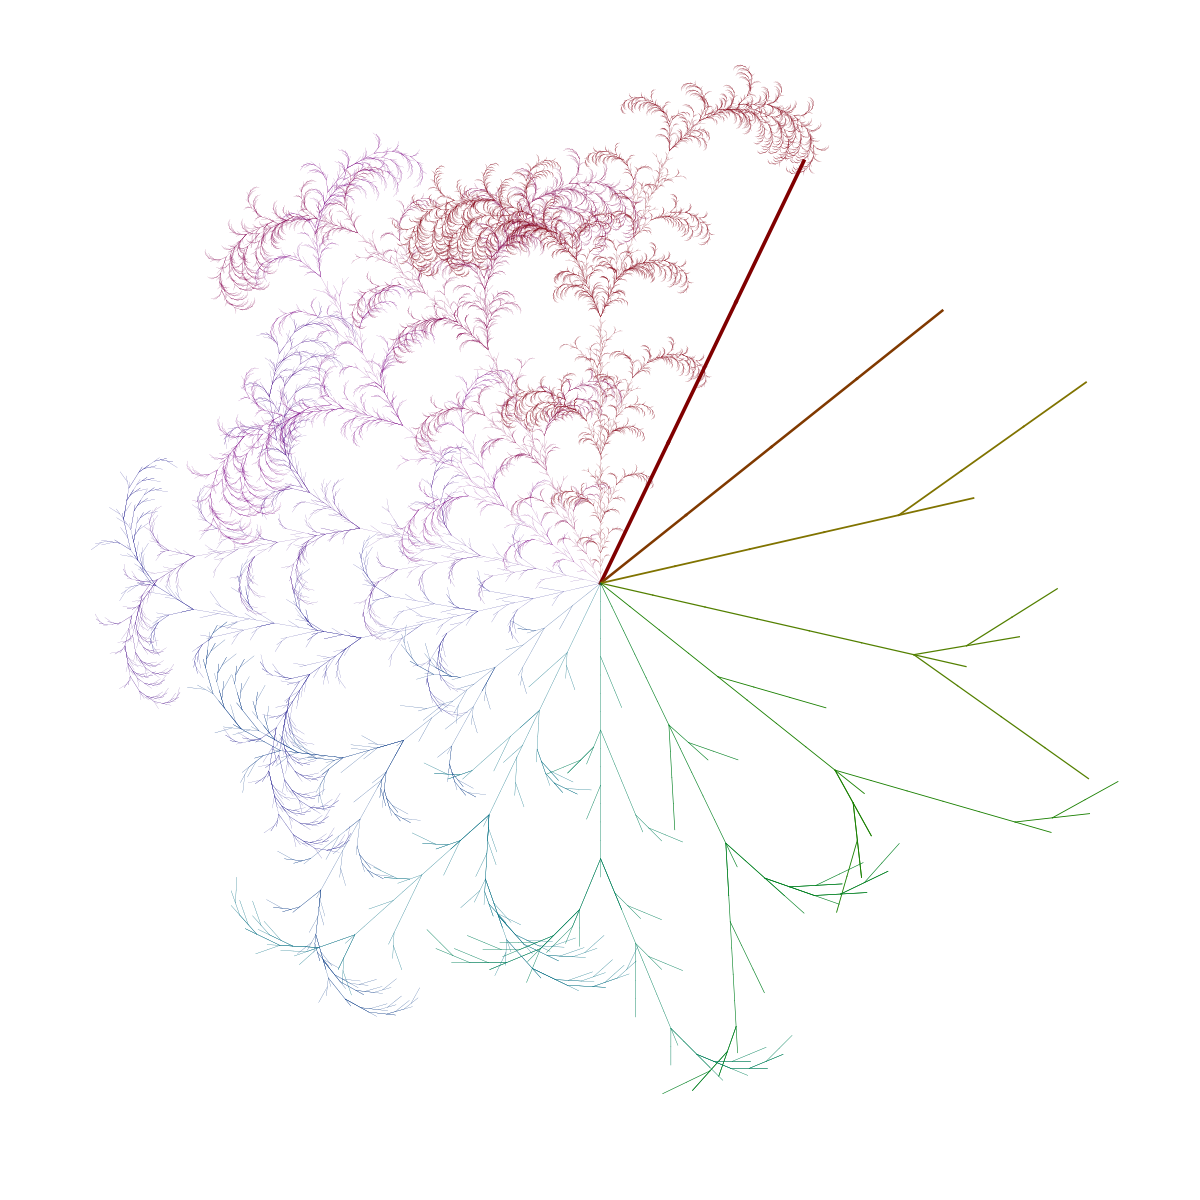
\includegraphics[height=10cm]{lsystem.png}
  \caption[The output of several L-systems]{The turtle evaluations of the different L-Systems given by $n=0,3...36,39$, as computed in Fig.~\ref{tab:example131b}. Consecutive systems are evaluated in a different frame, rotated clockwise from vertical. Each evaluation is drawn a factor of $0.7$ times smaller than its predecessor.}
  \label{fig:lsystemOutput}
\end{figure}

The result from these systems is generally pleasing given the compact description, and simulates a discrete form of growth as successive evaluations occur. The book \emph{The Algorithmic Beauty of Plants}\cite{ABP}, from which this example was taken, gives a very detailed introduction to the modeling of flora using L-Systems.
% and continues to introduce some standard extensions to the basic L-systems already described, including:

\begin{figure}
\[
\begin{array} { l l }
\multicolumn{2}{l}{$initial string$: A(0,0)}\\
\multicolumn{2}{l}{$production rules$ :}\\

1: & A(x,i) \rightarrow S(x)B(x,i)A(x+\Delta,i+1)\\
2: & S(x) \rightarrow @R(0,1,0,0,0,1)+(Y(x))\&(P(c))F(\delta(x))\\
3: & B(x,i): \{\\
   & \quad $if$ \; (i \% 2 == 0) \; \theta = 0;\\
   & \quad $else$ \; \theta = 90;\\
   & \} \rightarrow [/(\theta)L(x,i)R(x,i)]\\
4: & L(x,i) : \{\\
   &  \quad $if$ (i \% 2 == 0) \{\\
   &  \quad \quad angle = \varphi_L(x);\\
   &  \quad \quad length = h_L(x);\\
   &  \quad \} $else$ \{\\
   &  \quad \quad angle = (\varphi_L(x)+\varphi_R(x))*0.5;\\
   &  \quad \quad length = (h_L(x) + h_R(x)) * 0.5;\\
   &  \quad \} \rightarrow [+\;($angle$)\; $Organ$ \;($length$)]\\
5: & R(x,i):\{\\
   &  \quad $if$ (i \% 2 == 0) \{\\
   &  \quad \quad angle = \varphi_R(x);\\
   &  \quad \quad length = h_R(x);\\
   &  \quad \} $else$ \{\\
   &  \quad \quad angle = (\varphi_L(x)+\varphi_R(x))*0.5;\\
   &  \quad \quad length = (h_L(x) + h_R(x)) * 0.5;\\
   &  \quad \} \rightarrow [/(180)\;+\;($angle$)\; $Organ$ \;($length$)]\\
\end{array}
\]
\caption[An example of a complex L-system]{A parameterised programmable L-system from\cite{Anastacio09} to model the biological phenomena of decussate phyllotaxis. The necessity of referring to the previous iteration adds considerable complexity.}
\label{fig:notanlsystem}
\end{figure}

A basic L-system has several limitations, including a lack of environmental sensitivity, non-realistic rendering and a complex grammar editing process. To overcome these, L-systems have been periodically extended. The remainder of this section explores some of these extensions and their applications:

\begin{itemize}
\item{\emph{Context sensitive}. As described above, symbol replacement can occur based on the surrounding elements.}
\item{\emph{Stochastic}. Each production rule is given a corresponding probability with which it occurs on each iteration\cite{Yokomori80}. For example the branching characteristics of a tree may be encoded in a stochastic L-system\cite{Prusinkiewicz94}, or the choice of which building to place on a given parcel of land\cite{Parish01} may be made stochastically. While a basic L-system is deterministic in that it always creates the same output, a stochastic L-system may produce different output every time it is evaluated.}
\item{\emph{3D}. By using a three dimensional turtle, instead of the two dimensional standard, three dimensional geometry can be created. For example, \cite{Prusinkiewicz88} uses a two-axis rotation system to manoeuvre the turtle in 3D, while using L-system rules to determine the developmental cycles.}
\item{\emph{Parametric.} Here each symbol is given a set of parameters, and a replacement can only take place if a logical statement associated with the parameters is true \cite{Hanan92}. Parametric L-systems are comparable to the parallel case of attributed formal grammars\cite{Knuth68}. These parameters can model the flow of morphogens such as genes or hormones\cite{Buck05}.}
\item{\emph{Table}. These use a variable table of production rules to simulate step-changes in the applicable rules. For example one table may model the plant in a winter (non-flowering) state, and another the summer (flowering) state.}
\item{\emph{Map}. This early approach to produce a graphical interpreter for  L-systems uses a parallel grammar to manipulate a geometric graph as ``cells''\cite{Lindenmayer79}. Because this system works directly on geometry it is unnecessary to interpret the results using a turtle. Map L-systems are a geometric analog of graph grammars, see Sec.~\ref{s:ggrammars}.}
%\item{\emph{Programmable}. \cite{Anastacio09} Programmable L-systems also have a serial analog in programmed graph grammars.}
\item{\emph{Environmentally sensitive}. There has been a large quantity of work to allow L-systems to interact with their virtual environments. Table-L-systems provide a discrete phase-transition in response to external stimuli, while context sensitive L-systems give only topological self-sensitivity. L-systems that are physically constrained by their environment are introduced by \cite{Prusinkiewicz94}, although the effect of the plant on the environment are not modelled. To address this issue, bidirectional information exchange is introduced by \cite{Prusinkiewicz96}, using physical simulations to describe the availability of water and light to developing foliage and root systems. Geometrically self-sensitive L-systems are used by Parish\cite{Parish01} to generate road networks; these modify a production rule with both global goals and local geometric constraints.}
\end{itemize}

%Developmental models of hebaceous plants for computer imagery purposes\cite{Prusinkiewicz88} 3d turtles. Developmental models. L-systems for delaying flowering, or counting organs (such as leaves, flowers). parallel graph rewriting systems for repacing stems between branches.

%PARAMETRIC L-SYSTEMS AND THEIR APPLICATION TO THE MODELLING AND VISUALIZATION OF PLANTS.  Hanan's PhD thesis. \cite{Hanan92}. Introduces numerical parameters. Also parameters for deciding while rule to apply.

%Barley morphology, genetics and hormonal regulation of internode elongation modelled by a relational growth grammar. Simulates passing morphogens via parameters \cite{Buck05}

%PARALLEL GENERATION OF MAPS:DEVELOPMENTAL SYSTEMS FOR CELL LAYERS\cite{Lindenmayer79}. Map L-systems. Parallel application of graph-grammars. Unlabelled nodes, labelled edges, labelled cells. Forming closed cells of the plane. cells: Used to model ferns\cite{ABP}

%Table l-systems -> parametric L-systems, enviromentally sensitive l-systems, open l-systems (lgiht senstiive) -> self-sensitive l-systems (muller). Increasing levels of simulation / feedback Section ~\ref{s:simulation}

%Synthetic topiary \cite{Prusinkiewicz94} Exploring space using L-System. Environmentally sensitive parametric probabilistic stochastic L-Systems.Environmental sensitivity simulates ``pruning'' to constrain a plant to a boundary

%Visual models of plants interacting with the enviornments in\cite{Prusinkiewicz96}. Attempt at a universal environmental feed back mechanism - now sensitive to self and exterior conditions. Bidirectional information exchange between model and environment. Includes environemental response (such as \cite{Greene89} - voxels) in L-systems. Sensitive to moisture or light, no collision.

%Procedural modeling of cities\cite{Parish01}a different kind of context sensitivity - for the turtle rather than the grammar. two types of l-system for street layout and mass models. Good first pipeline for top-first procedural generation. Extended L-systems context sensitive by parameter assignment by a global goal, then a local constraint takes over.

% not used: The FL-system: a functional L-system for procedural geometric modeling \cite{Marvie05} terminal symbol, and symbol age. programmed in that conditional statements can chosoe the next rule ot be applied. stochastic, parametric context free L-system. Operations Manipulate local frame instead of moving a turtle, and  insert geometry at these locations. Some commands to delay parallel execution to the end (half a chomsky?) 

% \cite{Anastacio09} Plant modeling. sketches to models (reconstruction!). example of a parametrised, programmable stochastic L-System. Good example of complex L-system.

As they have been extended to overcome their limitations, L-systems have become increasing complex. One case study is that of phyllotaxis, the pattern that plant organs (leaves or flowers) form around the stem; in particular decussate phyllotaxis alternates between pairs of leaves at $90^\circ$. It is instructive to compare an L-system for a phenomena such as decussate phyllotaxis from Fig.~\ref{fig:notanlsystem}, to the same description in a general purpose language, Fig~\ref{java}. It becomes clear that it is more complex to represent this phenomena in parallel production systems than in Java. This suggests an issue for the designer of the L-system in comprehending the consequences of an edit to an L-system. To address this usability issue, there is limited work to  reconstruct L-systems from an image representations \cite{Vstava10,Shlyakhter01} or user sketches\cite{Anastacio09}, avoiding the issue of writing grammars altogether. 

The above argument suggests L-systems are an over simplification of botanical systems, that are not gracefully extended to all observed plant models. It is strengthened by recent research into \emph{physical simulation} to model the Auxin hormones that cause phyllotaxis\cite{Smith06}. More generally, algorithmic botany has moved away from L-systems, towards deeper physical simulations such as the simulation of tropisms in \cite{Palubicki09} or geometric simulation of the apical meristem (growing tip of a plant shoot) in \cite{Nakielski00}. 

There are similarities between programming an L-system and \emph{multicore} (parallel) programming. In particular the current string is reminiscent of the \emph{shared state} of some parallel models of computing, and developmental delay\cite{Prusinkiewicz88} is similar to \emph{message passing}. The similarities suggest that some of the problems of multicore programming may be present when designing large L-systems. These may include synchronisation issues, dead and live locks, as well as race conditions.

\section{Shape Grammars}
\label{s:shapegrammars}

In the previous sections we have examined grammars that are formed by production rules over strings of symbols (formal grammars and L-systems), as well as graphs. In contrast, \emph{shape grammars} consist of production rules that match and replace certain \emph{shapes} in a figure. The high level description of the grammar remains the same --- a start state is given, and production rules transform it to a shape in the language; however the states and rules are expressed as shapes rather than graphs or symbols. 

Stiny and Gips created the concept of shape grammars in 1971\cite{Stiny71}. They have since been used in a relatively unchanged form to design a wide range of procedural models within academia. We may position shape grammars in our spectrum of proceduralisation by noting that like L-systems they are constrained to the construction of geometry. They are also Turing complete\cite{Gips99}. 

In comparison to L-\emph{systems}, shape \emph{grammars} are indeed grammars. They specify a language, a set of valid statements, but do not say which specific sentence should be generated at a particular evaluation. The order of the rules applied may be determined manually or automatically depending on the application.

The formalism behind a shape grammar eventually\cite{Stiny80} came to consist of a set of shapes, $S$, a set of symbols, $L$, an initial labelled shape, $\gamma_0$, and a set of production rules, $R$; each production rules takes the form $\alpha \rightarrow \beta$. The left hand side, $\alpha$, specifies zero or more labelled shapes, $(S,\; L)^*$, that are matched against the current shape. The right hand side, $\beta$ gives a labelled or unlabelled replacement, $\in\;(S,\;L)^+\cup S+$. As with the previous grammars, we begin with $\gamma_0$, applying rules until all symbols have been removed. At this point the current shape, $\gamma$ is an element in the language defined by the grammar. 

In contrast to L-Systems, the production rules are not applied in parallel to all matching instances, rather in a serial manner reminiscent of Chomsky grammars\cite{Chom56}. Given the lack of restrictions on the context of the shape, we may see similarities to a type-0 Chomsky grammar. 

An example of a very simple \facade{} shape grammar is given in Fig.~\ref{fig:myShapeGrammar}, left, using the symbols $L = \blacktriangle,T$. We show the evaluation of one shape in the language in Fig.~\ref{fig:myShapeGrammar}, right, by repeated production rule application until no symbols remain. Various other shapes in the language are shown in Fig.~\ref{fig:myGrammarResults}.

\begin{figure}
\centering
\def\svgwidth{1.\columnwidth}
\includesvg{11-readings/images/myShapeGrammar}
\caption[A simple \facade{} shape grammar]{\label{fig:myShapeGrammar} Left: We introduce a shape grammar consisting of 8 shape rules. The shapes on the left of each arrow may be replaced by the shapes on the right of the same arrow. Right: An example derivation of this shape grammar that creates a bungalow. The number of applications of a rule are specified in parentheses.}
\end{figure}

\begin{figure}
\centering
\def\svgwidth{0.8\columnwidth}
\includesvg{11-readings/images/myGrammarResults}
\caption[Evaluations of a shape grammar]{Four evaluations of the shape grammar given in Fig.~\ref{fig:myShapeGrammar}, with the rules that created them. 
%The numbers in parenthesis indicate the number of applications of a single rule.
}
\label{fig:myGrammarResults}
\end{figure}

A single grammar production rule can often be matched to an infinite number of positions on the current shape by matching \emph{subshapes}. For example a rule containing an arc may be positioned at an infinite number of points around a circle, as in Fig.~\ref{fig:ggTree}.

\begin{figure}
\centering
\def\svgwidth{0.8\columnwidth}
\includesvg{11-readings/images/ggTree}
\caption[The use of shape grammars to position trees on an circle]{Left: A shape grammar production rule that positions a tree on an arc. Right: If we allow subshape matching under rotation we may position trees at an infinite number of locations on a circle. We show the result of several applications of the production rule upon a circle.}
\label{fig:ggTree}
\end{figure}

Given this flexibility of rule application, it is a natural that the categorisation of the different varieties of shape-grammars concerns itself with the mechanism for matching $\alpha$ against the current shape, $\gamma$, the \emph{subshape problem}. Common variations include:

\begin{itemize}
\item the shapes that may be matched --- such as only lines, rectangles or curves in 2D or 3D,
\item the type of matching that occurs --- whether only whole shapes (such as rectangles), or \emph{subshapes} (such as one corner of a rectangle), may also be matched. The advantage of subshape matching is that it allows more ``emergent'' (unexpected) shapes to be generated, 
\item the transform we are allowed to apply to $alpha$ to locate a match --- such as isometries, rigid transforms or affine transforms, and 
\item whether any parametrisation of $\alpha$ is allowed.
\end{itemize}

These \emph{parametric shape grammars}\cite{Stiny80} are variants which allow the arbitrary parametrisation of production rules. We show an example parametric rule in Fig.~\ref{fig:paramShapeGrammar}. There are no computational limits placed on these rules, and are typically expressed in the corpus by prose\cite{Stiny77}, or omitted entirely\cite{Flemming:1987:MTS}. These parametrisations can be also used to limit the repetition of rules, for example by adding area or height conditions. 

\begin{figure}
\centering
\def\svgwidth{0.8\columnwidth}
\includesvg{11-readings/images/paramShapeGrammar}
\caption[A parametric shape grammar production rule]{A single parametric shape grammar production rule inspired by\cite{Stiny80}. The accompanying schemata might specify that the new point $(x_6,\; y_6)$ lies on the line between existing points $(x_1,\; y_1)$ and $(x_2,\; y_2)$, and similarly for the other new points. This parametrisation permits a language of nested pentagons to be defined.}
\label{fig:paramShapeGrammar}
\end{figure}

%%%%%%%%%%%%%%%%%%%%%%%%%%%%

%variations: are shape grammars are serial or parallel (\cite{Gips75} was parallel, but was an exception). In early work\cite{Stiny71} these symbols were unique shapes, although later because parts of entire shapes, or subshapes. Perhaps this is related to the fact that many of the early grammars were evaluated manually.

The computational complexity of finding potential matches of $\alpha$ in the current shape, $\gamma$, the subshape problem, is well studied. The matching of whole labelled shapes has a linear computational complexity in the number of the current shapes.
Therefore there are well developed algorithms and systems for matching rectilinear\cite{krishnamurti81,Krishnamurti80} and curved 2D shapes.
However parametric subshape recognition is NP-hard\cite{Yue09}, even in the case of a rectilinear shape vocabulary. This has not stopped implementations of the parametric case in 2D\cite{Mccormack02}. 
The theory of shape recognition in 3D is addressed by \cite{Krishnamurti92}, against straight line figures only, while \cite{Chau04} introduces an implementation that limits their use to circles and arcs. The issue of subshape matching with general curves and surfaces in 3D is still unaddressed in the literature.

%The arithmetic of shapes\cite{Krishnamurti80}. First shape grammar interpreter - subshape recognition (limiuted to using euclidean transorms to entire shape). 
%The construction of shapes\cite{krishnamurti81}. More theory for the above paper

%Shape recognition in three dimensions\cite{Krishnamurti91}. Subshape problem solution in three dimensions. Situations in R3 in which we can match points. straight lines only. No analysis of more complex curves.

%Because of these complexity problems, there have been attempts to use graph grammars as the data structure\cite{Yue09}, and these have been applied to the classic Palladian grammar\cite{Grasl10}. While these conversions improve the complexity of the subshape problem, the issue of termination critera, below,  remains.

%Shape Grammars and Their Uses\cite{Gips74}: Gipps thesis. presents colon image generation and equivilence to a turning machine. 

%Evaluation of a 3D shape grammar implementation. 3d shape grammar, coke bottles through the ages. \cite{Chau04}. Concept of maximal shapes explained (where first?), to give a shape representation of a particular geometry. ``A basic element is said to be maximal with respoect to another basic element if and only if it cannot be combined to form a single basic element'' General analysis of matching criteria for solids and surfaces in 3 or higher dimensions is missing

%Computer implementation of shape grammars\cite{Gips99}. Shape grammars are turing complete. Good range of problems/issues with shape grammars in 1999. 

%Computation friendly shape grammars\cite{Yue09}. Different classes of shape grammars - (2d || 3d) (rectilinear || with curves) (non-parametric || parametric )Proves NP-hard to perform parametric subshape recognition for an arbitrary number of open terms. Observes that some examples do no depend on emergent shapes (everything is labelled). (later becomes split shape grammars). Suggests a different interpretors for different subcalsses of parametric shape grammars. Connection between graph grammars and shape grammars (examples given for ice ray). Unclear why this isn't NP-hard again (clique problem) - relies on labels to avoid this complexity?

%Palladian Graphs\cite{Grasl10}. Shape bounds using graphs (Yue09 esque). Single Push Out graph rules. Attributed nodes (symbols and integer values) Converted Palladian Grammar (Stiny78) to a graph grammar. ``state node'' to model execution order. undrirected multigraph with node labels. Some of the same issues as original palladian grammar. This search space isn't described in the paper. User specifies each of the rule application. Claim that random generation works over this.

%supporting designers hierarchies through parametric shape recognition\cite{Mccormack02}. Shape grammar interpreter using paraemtric subshape recognition.claims to be first parametric features. Heuristics for faster matching (a hierarchy of shape classes by feature invariance to various transforms)  - may still fall back on exhaustive search.

%%%%%%%%%%%%%%%%%%%%%%%%%%%%

Despite these complexity issues, shape grammars have been widely applied in academia. The initial examples were artistic drawings\cite{Stiny71} and 2D architectural plans\cite{Stiny78}. These were extended to 3D isometric plans of houses, generated using parametric shape grammars\cite{Koning81}. 3D shape grammars are less common, and tend to be simple, such as modeling historic soft drink bottles\cite{Chau04}. A wide range of applications have been found for shape grammars include modeling the morphospace of chair-backs\cite{Knight80}, Harley Davidson motorbikes\cite{Pugliese02}, and coffee machines\cite{Agarwal98}.

%The language of the prairie: Frank Lloyd Wright's prairie houses\cite{Koning81} EnP:B. Tree of possible resulting hosues. Isometric. Based around fire palce. Dubious attempt at creating roofs for arbitrary houses uses shape grammars. Parameterization omitted (as evar!)

%Capturing a rebel: modeling the Harley-Davidson brand through a motorcycle shape grammar\cite{Pugliese02}. Capturing a brand. 45 rules. 2D.  Manual evaluation. Parametrically constrained. Comparison of Harley-esque and non-Harley-esque constraints via user studies.

%More than the sum of its parts: the grammar of Queen Anne houses\cite{Flemming:1987:MTS}. 3D. Grows floorplans upwarsd using rectilinear extrusions.

%Creating cross-over vehicles: Defining and combining vehicle classes using shape grammars\cite{Orsborn06}.

A subtlety of shape grammars are their termination criteria. The language specified by the grammar does not contain all possible evaluations of rule sequences, but only those shapes that do not contain symbols. There are sequences of production rule applications in Stiny's well cited Palladian grammar\cite{Stiny78} that lead to dead-ends in which the grammar can never terminate, Fig.~\ref{brokenPalladian}. Of particular issue is the fact that there are no guarantees as to how many times we might have to evaluate statements in the grammar before a valid result in the language is generated.

\begin{figure}
\centering
\def\svgwidth{0.8\columnwidth}
\includesvg{11-readings/images/palladianGrammar}
\caption[Dead ends in the Palladian grammar]{\label{fig:palladianGrammar}Top Left: An example from Stiny's Palladian shape grammar\cite{Stiny78}. Bottom left, right: Example rule sequences in the same shape grammar that lead to dead ends. After these rules, there is no way to remove the symbols \textbullet, or \emph{O}, leading to evaluations of the grammar that are not in the language.}
\label{brokenPalladian}
\end{figure}

The lack of a mechanism to specify situations in which a rule cannot be applied causes additional difficulties with self intersection and termination (\emph{negative application conditions} in graph grammar terminology). A shape grammar rule with a $\beta$ that is a superset of the corresponding $\alpha$ gives rise to an infinite language. We present an example in Fig.~\ref{fig:myGrammarResults}d, in which the \facade{} may be indefinitely tall. This poses the problem of how to stop a sequence like this from intersecting other geometry, especially in non-parametric shape grammars.

Because of the requirement for shapes in the language to not contain symbols, and the infinite nature of certain shape grammars, we may characterise shape grammars as a search through some shape-space. The order of search can either be manually defined (as in most of the corpus) or automated to produce figures automatically\cite{Grasl10}. Regardless of the mechanism for choosing rules, sequences of rules will behave in one of the following ways:

\begin{itemize}
\item All symbols will be removed, and a figure that the grammar describes will be produced.
\item Symbols remain in the figure, but no further rules may be applied. The evaluation stalls at this invalid shape (Fig.\ref{fig:palladianGrammar}).
\item The evaluation continues endlessly. Either by force or choice the sequence of applied rules is unending, and evaluation continues indefinitely. There are similar situations in formal grammars, graph grammars and L-systems.
\end{itemize}

Other common issues surrounding the use of shape grammars are well summarised by \cite{Gips99}, for example
\begin{itemize}
\item the subshape and termination problems introduced above,
\item the design of an adequate interface for the construction and application of shape grammars, 
\item the lack of robust implementations for parametrised shape grammars, 
\item the difficulty in application to non-linear geometry, such as curved surfaces, 
\item the lack of a standardised shape-description, and finally,
\item the lack of production grade or commercial systems for working with shape grammars. 
\end{itemize}

\section{Split Shape Grammars}

The computational complexity of classical shape grammars seems to have limited their use to small scale academic projects. However in 2003, Wonka et al. created a specialisation of shape grammars, \emph{split shape grammars}\cite{Wonka03}, with lower complexity. To simplify their computation, these extend set grammars, initially within a 2D domain of labelled nested shapes and using only whole-shape matching. These grammars have been shown to be well suited to large urban environments, and \facade{} generation in particular. 

As the name implies, a split shape grammar consists of production rules that take a labelled shape and split it into a number of covering labelled shapes. Unlike a shape grammar these labels are categorised as terminal or non-terminal. This delegation of area to subsequent rules continues down a hierarchy until only shapes with terminal symbols remain.

A principle assumption is that this hierarchical split operation is well suited to the generation of designed structures. There is ample justification for this assumption in the literature of early urban modeling pipelines, such as the book \emph{A Pattern Language}\cite{APL}, which introduces a hierarchy of 35 guidelines for the design of of urban areas, ranging from ``major city structures'' and ``common land'' to ``structure of the floor and walls'' and ``furnishing'':

\quote{The elements of this language are entities called patterns. Each pattern describes a problem which occurs over and over again in our environment, and then describes the core of the solution to that problem, in such a way that you can use this solution a million times over without ever doing it the same way twice.}

The book is representative of the architectural literature in that it purports to present solutions to urban design problems, without providing sufficient details for an computational implementation, for example: 

\quote{Pattern 10...Do this by means of collective regional policies which restrict the growth of downtown areas so strongly that no one downtown can grow to serve more than 300,000 people.} 

%However there are insufficient details for an automated implementation \cite{APL}:
%As a side note, we note Hillier's observervation that architectural theory books are often insufficiently detailed to be of use in the field of urban PGM\cite{SITM}:
%\quote{An architectural theory, as we see it, should deepen our grasp of architectural phenomena, and only subsequently and with great modesty, suggest possible principles on which to base speculation and innovation in design.}

This hierarchical split approach to urban languages presented by \emph{A Pattern Language} is quite pervasive in the computer graphics literature, with examples such as \cite{Finken08}, \cite{Hahn06}, \cite{Aliaga07},  and \cite{Parish01} using variations on the theme of a hierarchical urban decomposition.

% \cite{Finken08} Detailed Building Facades Some type of hierarchicial classification (not split shape, but fodder?)

%Persistent realtime building interior generation\cite{Hahn06}. Generated and destroyed as required.

Returning to Wonka's 2003 paper\cite{Wonka03}, we observe that this concept of a strict hierarchy in urban design is exploited to simplify shape grammars.

Compared to shape grammars, split shape grammars have the advantages of fast computation and no dead-ends during the evaluation. The subshape problem is bypassed by using a set grammar\cite{Stiny82} in which matching takes place based on a whole shape and a symbol. This removes the emergent behaviour of subshape matching, but permits finding all possible shape matches in time linear to the size of the existing figure. While certain split shape grammars may be evaluated endlessly, if they do terminate they are guaranteed to supply a valid shape.

M\"{u}ller et al.'s later influential paper, \emph{Procedural Modeling of Buildings}\cite{Pascal06}, extends the concept of a split shape grammar to 3D and introduces a written formalism for split shape grammars, \emph{CGA Shape}. The system has gained widespread use and notoriety as it has been successfully commercialised\cite{cityEngine}.

A CGA Shape grammar consists of an initial labelled shape and a set of production rules, each with a certain priority. All the applicable rules with the highest priority are executed before others; this priority mechanism is exploited to produce differing geometry based on the required level of detail. Models with higher details are generated by executing rules with lower priority. 

To define the reference frame for the production of geometry, a scope is introduced that defines a frame, as well as an extent, as in Figure~\ref{fig:cgaScope}. This is reminiscent of an L-system's turtle. When geometry is created, the scope defines the size, location and orientation. When the current shape is split, the scope defines the orientation and number of splits.

\begin{figure}
\centering
\def\svgwidth{0.8\columnwidth}
\includesvg{11-readings/images/cgaScope}
\caption[CGA Shape's scope]{The current scope in a CGA Shape grammar defines a frame and extent for the production rules. Given the initial 3D scope, shown in the top left, and the initial geometry, top middle, we show the result of three production rules. Rule one translates and scales the frame before adding another hexagonal prism of dimension specified by the transformed frame. Rule two performs a component split, creating 2D faces, giving them each their own 2D frame. Rule three subdivides the current shape along the x axis into 3 equally high prisms, and matching scopes. }
\label{fig:cgaScope}
\end{figure}

A production rule of a given priority in CGA Shape consists of a unique ID, a parametric symbol to match on, an optional condition, a labelled successor shape that is generated, and a probability with which the rule will be applied: \emph{id: predecessor : cond $\leadsto$ successor : prob}. The successor operation has an involved syntax that is able to manipulate the scope via transforms, splits, repeats and dimension reduction. A 2D example is given in Fig.~\ref{fig:splitGrammar}. The condition is used to limit the applicability of the rule, for example to shapes of a certain size, or if certain occlusion conditions are met. These occlusion queries form a domain-specific environmental sensitivity that is used, for example, to stop the production of windows occluded by roof geometry. This is the only context sensitivity available in the system.

\begin{figure}
\centering
\def\svgwidth{0.8\columnwidth}
\includesvg{11-readings/images/splitGrammar}
\medskip
\begin{tabular} {ccl}
&&\\
1:&\facade&$\leadsto$ Subdiv(``X'', 2, 0.2, 1r, 1r)\{l\textbar a\textbar u\textbar u\}\\
2:&u& $\leadsto$ Repeat(``Y'', 1.5)\{w\}\\
3:&l&$\leadsto$ Subdiv(``Y'', 1.5, 1.5, 1.5, .1.5)\{w\textbar d\textbar w\textbar w\}\\
4:&w&$\leadsto$ Subdiv(``X'', 0.3, 1r, 0.1)\{wt\textbar wm\textbar wb\}\\
5:&d&$\leadsto$ Subdiv(``X'', 1r, 0.3)\{dt\textbar dm\}\\
6:&wm&$\leadsto$ Subdiv(``Y'', 0.15, 1r, 0.15)\{wl\textbar wc\textbar wr\}\\
7:&dm&$\leadsto$ Subdiv(``Y'', 0.15, 1r, 0.15)\{dl\textbar dc\textbar dr\}\\
8:&wc&$\leadsto$ I(``window'')\\
9:&dc&$\leadsto$ I(``door'')\\
\end{tabular}

\caption[The evaluation of a split shape grammar]{The production of a \facade{} in CGA, top, via the given grammar, bottom. Rule 1 splits the \facade{} into 3 floors and a architrave (top middle). Rules 2 \& 3 create repeating windows and doors according the floor (top right), while rules 4--7 further refine the window and door positions. Rules 8 \& 9 position geometry to create the doors and windows (middle right).}

\label{fig:splitGrammar}
\end{figure}

%split from 3 to 2 dimensions (but not to 1 dimension?) turtle-like frame movement. conditional application (self interseciton). levels of priority (LOD). evaluation order:? inserting meshes. marks old shapes as ``inactive''. prbabilitstic abs/rel scaling. 

Split shape grammars have been successfully applied to the reconstruction of  several historical sites such as Mayan ruins\cite{cga_puuc}, the ancient Roman city of Pompeii\cite{Muller05,Dylla08} and Malay houses\cite{Said08}. Novel uses of split shape grammars include the presentation of uncertainty in archaeological findings by presenting several derivations of a grammar\cite{Haegler09}, and animatable articulated objects structures\cite{Ilvcik10}. 

%Procedural 3D reconstruction of Puuc buildings in Xkipche\cite{cga_puuc}
%Procedural modeling for digital cultural heritage: reconstruction. not cga shape! useful reference for somewhere?
%Procedural Skeletons: Kinematic Extensions to CGA-Shape Grammars\cite{Ilvcik10}.CGA shape for animation. example of digger. Automatic kinematic hierarcy updates. Adresses problem of maintining a bone system throught an otherwise serperate hierarchy -by linking leaf nodes of the parse tree at each step.
%Rapid Procedural-Modelling of Architectural Structures.

Writing the production rules for split grammars is somewhat involved and required specialist knowledge. 
%Early attempts for shape-grammar like systems, such as ChemTrains required 
Several attempts have been made to simplify the process. The first presents the production rules as a graph\cite{Patow12}, giving an understanding of the relationship between application possibilities of the rules. However using this system requires the user to comprehend the underlying grammar before using it. An alternative is given by Lipp et al.\cite{Lipp08}, who allows the user to construct a grammar by editing an example instance. By constraining the modeling tools to those that may be translated to production rules, the user is able to quickly produce a PGM without interacting with the grammar itself. When a user edits a single feature in an example instance, this edit must be encoded into the grammar, in a persistent manner. To do this Lipp introduces \emph{instance locators} to store user edits in a split shape grammar, Fig~\ref{fig:instanceLocator}. 
%Interactive visual editing of grammars for procedural architecture \cite{Lipp08} 
%\cite{Bell92} ChemTrains rule based shape-grammar esque editor for pictorial simulations.


\begin{figure}
\centering
\def\svgwidth{0.6\columnwidth}
\includesvg{11-readings/images/instanceLocator}
\caption[An instance locator]{The instance locators of Lipp et al. \cite{Lipp08} identify a component by its position in a derivation tree (left). After each production rule the index referred to (dashed lines) can be stored relative to the start, middle or end of the split sequence. The instance locator can be used to store modification to a procedural object, such as a modification to the style of a window, right.}
\label{fig:instanceLocator}
\end{figure}

%User-Friendly Graph Editing for Procedural Modeling of Buildings\cite{Patow12} Interactive technique for editing shape grammars. Similar to the visual graph editing system for city Engine. Basically uses the same shape grammar. Has exceptions to rules, to replace a specific element. Multiple inputs seems to exist as it's based on a DAG, but are not addressed in detali. Discusses graph based applications.

Strict hierarchy and \emph{over-compartmentalisation} can cause problems when working with shape grammars\cite{Hohmann09}. For example sharing information about the number of elements in a \facade{}, as in Fig.~\ref{fig:hierarchyClash}, left. Additional difficulties are caused by problems placing objects over two or more disjoint portions of the hierarchy, as in Fig.~\ref{fig:hierarchyClash}, right.  In these situations it is necessary to re-write the grammar to add a new shape, or to add some portion of the shape to two separate portions of the hierarchy. Recently work has begun to address this issue by creating connection patterns between portions of two different shape grammars\cite{Krecklau11}. 
The problem of over-compartmentalisation is uniquely critical to split shape grammars; while some shape grammars do use such a hierarchy\cite{Stiny78}, many do not\cite{Liu:2005:BCA,Koning81}. 

% The complexity of production rules in a real-life system is also problematic. 

%Procedural Modeling of Interconnected Structures\cite{Krecklau11}Extends CGA shape. Only 2 inputs. Manually coded correspondences between different parts of the structure. Geometric queries to shoot rays to recievers. Without any hit it fails.


\begin{figure}
\centering
\def\svgwidth{0.8\columnwidth}
\includesvg{11-readings/images/hierarchyClash}
\caption[The over-compartmentalisation problem in shape grammars]{Left: The strict hierarchy may cause problems for coordinating features, as in this evaluation of the grammar of Fig.~\ref{fig:splitGrammar}, showing a lack of synchronisation between the ground floor and upper windows. Right: The over-compartmentalisation means that it is impossible to place some features that cross over the hierarchy's bounds, such as positioning an intercom near the door (black rectangle).}
\label{fig:hierarchyClash}
\end{figure}

%Building chinese ancient architecture in seconds\cite{Liu:2005:BCA}. Shape grammar. contrstructive ``like lego''

% Language variations -- all different types of programming
% 
% Visual geometric programming -- introduce via non-geometric programming. Admit that it's in the wrong place wrt formal grammars.

\section{Data Flow Programming}
\label{s:dataFlowProgramming}

\emph{Data-flow graphs} are a model of parallel computation introduced as an alternative to the classical von Neumann model. 

Written imperative programming languages are typically a 1D sequence of symbols which explicitly sequence instructions. This ordering of instructions is typically associated with the von Neumann model, which executes a single instruction at a time. In contrast, a parallel model of computation may execute many instructions concurrently.

To schedule the execution of a single instruction, a general requirement is that the instruction's inputs are available --- whether they have been entered by the user or calculated by a previous instruction. The necessity of the inputs' availability creates a dependence of the following instruction on the previous instructions' execution, and may be represented as a data flow from the previous function to the next, as in Fig.~\ref{fig:dataFlowIntro}. In this way data flow languages are declarative, allowing the executing system's scheduler to determine the order of operations given the data flow constraints.

\begin{figure}
\centering
\def\svgwidth{0.4\columnwidth}
 \includesvg{11-readings/images/dataFlowIntro}
\caption[A data flow graph]{A data flow graph that calculates $ab+cd$ given the mathematical convention that multiplication instructions are performed before addition. The circular nodes are instructions, while the directed edges are the data flows. An inbound edge is an input to the instruction, while an outbound edge is a use of the output. Each instruction requires that all of their inputs be present before calculating an output. For example instruction 3 requires both instruction 1 and instruction 2 to be complete. However the order of the operations are not specified in a data flow graph, so the execution order may be 123, 213 or instruction 1 and 2 may be executed in parallel before 3.}
\label{fig:dataFlowIntro}
\end{figure}

We introduce data flow languages, and in particular graphical data flow languages for geometry as a typical example of a general non-written PGM system, before looking at an example commercial application. The topic of data flow programming occupies a wide range of our procedural spectrum. A data flow language with loops may be Turing complete, and has many applications from parallel programming to task scheduling. However there are a number of implementations that are graphical and geometrical --- their user interface is a graphical graph editor, and their output is geometrical. These are the use cases that are of most interest to PGM, being of similar generality to shape grammars, being concerned with the graphical domain. 

There are several varieties of data-flow graphs in the literature, we shall briefly examine the \emph{token based} model of Dennis from \cite{Dennis74}, introduced in 1974. Fig.~\ref{fig:myDataFlow} shows an example graph for generating nested rectangles, showing examples of splitting and combining data flow arcs. A token based data flow model models the arcs in data flow graphs as FIFO queues of tokens. Each token is associated with a value, in our example this value is either a rectangle or a Boolean. When a node has a token available on each of its inputs it removes these tokens from its input arcs, computes an output, and adds a token representing this output to any output arcs. The FIFO queues may be initialised with tokens before the system is executed (as Fig.~\ref{fig:myDataFlow}e). Ensuring that the correct sets of input tokens arrive at the front of the FIFO queues at the same time is challenging for the user, as demonstrated by the involved select/distribute syntax of our example. This \emph{sequencing issue} is one that will occur frequently in data flow graphs.
% solutions as to how we repeat things.

We note that the graph of Fig~\ref{fig:myDataFlow} can only be used for the generation of one figure at a time because of loops, negating the advantages of parallelism. This is somewhat mitigated by the use of tags\cite{Dennis74,Watson79}, in which each invocation of the graph uses tokens with different tags, allowing the same instruction node to execute on different sets of input concurrently.

\begin{figure}
\centering
\def\svgwidth{1.\columnwidth}
\includesvg{11-readings/images/myDataFlow}
\caption[A token based data flow graph]{A token based data flow graph (left) that generates nested rectangles (right). The data flow graph takes an input rectangle (a), shrinks and positions it (b) or terminates if the area is less than a constant (c), otherwise the sequence repeats itself. The sequencing issue of whether to take a new input rectangle, or iterate on the existing is addressed by the select and distribute nodes. The select node (d) outputs either the new input rectangle, or the result of a previous iteration, based on the horizontal input; it is initialised with a token of value false (e) to initially take a new input rectangle. The distribute node (f) sends the output of the shrunk rectangle to one of two locations, based on the result of the area test. It is either discarded (g), or output (h) and used in a subsequent iteration via the select node (d).}
\label{fig:myDataFlow}
\end{figure}

An alternative data flow model offers a different way to mitigate the sequencing issue, by removing loops from data flow graphs. The \emph{structural data flow} model\cite{Davis82} models arcs as arbitrary and possibly infinite data structures. As computations are completed, these data structures are updated, and their values used by subsequent nodes. Structural data flow diagrams do not require loops as the token based systems do, however this comes at the cost of storage; all computed values are retained by the data structures. Additionally nodes must be equipped with the logic to comprehend the, possibly involved, input data structures. 

%CAJOLE\cite{Hankin81} asked users to use tail-end recursion instead of iteration, this avoided allowing cycles in the graph. Others introduced some sort of loop variable that could be accessed. used in Id and Lucid.

%%%%%%%%%%%%%%%%%%%%%%%%%%%%%%%%%%%%%%%%%%%%%%%%%

%Data-driven nets: Davis. The original citation?
%Data Flow Program Graphs, IEEE computer. Keller, DAvis\cite{Davis82}. Introduces the token and structure models. tokens control data flow. macrofuntions as routines. cyles in graphs.

%The two different rationals behind data flow programming, parallelism and east of use, lead to textual and graphical interfaces developing in parallel. In addition to the parallelism argument for data flow programming, ease of use was also a motivating factor.


While textual systems, such as LAU\cite{Plas76} and CAJOLE\cite{Hankin81}, focused on parallelism and efficiency, another early justification for data flow programming was ease of use. Curiously the development of easy to use graphical user interfaces to data flow languages preceded these formal written languages. In particular Sutherland introduced a data flow editor\cite{Sutherland66} in 1966, 8 years before Dennis' work. This system used a light-pen to edit the structure of data flow graphs, and define functions by drawing nodes and arcs. There followed many graphical data flow research languages, with examples such as the Graphical data-driven Programming Language\cite{Davis81} and Grunch\cite{Jong82}, a graphical interface to CAJOLE. Many of the graphical programs were more visually complex than their textural counterparts. In particular embedding a data flow graph into the plane often leads to the crossing (without connecting) of graph arcs, making reading the graph quite difficult. However this did not stop the use of graphical data flow languages in industry, with systems such as Prograph\cite{Matwin1985} for general programming and LabVIEW\cite{labview} as a digital laboratory, Fig~\ref{fig:labview}.

\begin{figure}
\centering
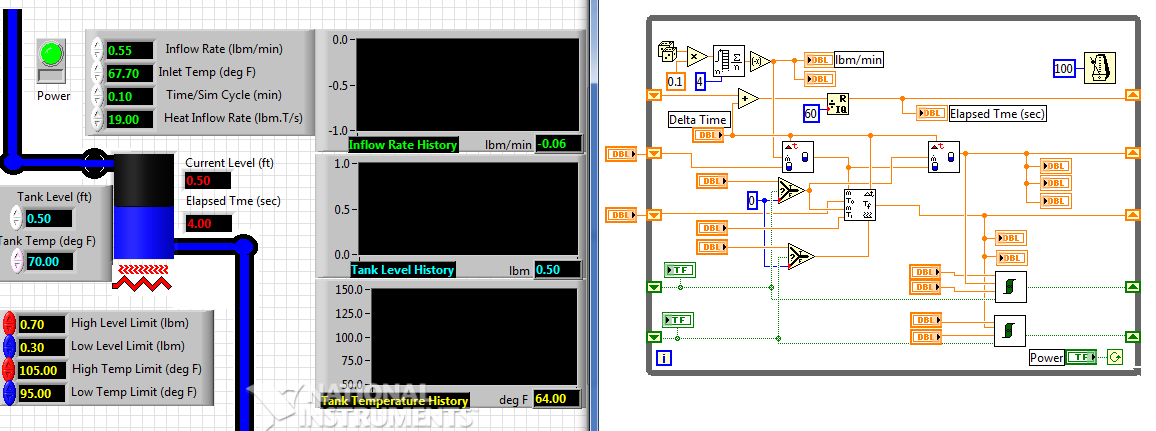
\includegraphics[width = 0.8\columnwidth]{labview.png}
\caption[The Labview graphical data flow language]{A visual data flow diagram used for controlling the temperature of a virtual water tank.}
\label{fig:labview}
\end{figure}

There are several interesting diversions at this point that are beyond the scope of this chapter:

\begin{itemize}
\item Data flow graph editors cannot express anything more than a written language (at their most expressive they are still only Turing complete) despite their additional dimensions. However many authors make the claim that graphical programming is easier as it is more difficult to introduce syntax errors than when writing text based programs.

\item There are a significant number of graphical editors for imperative  programming\cite{Tanimoto86,blockly}. These exploit the ease of use of graph-based systems to appeal to, for example, those new to programming. For example Scratch\cite{Resnick09} shown in Fig.~\ref{fig:scratch} is able to create geometry. These control graphs describe the sequence of operations, rather than the data dependencies, usually allowing side effects and mutable data structures which data flow programming largely avoids.

\begin{figure}
\centering
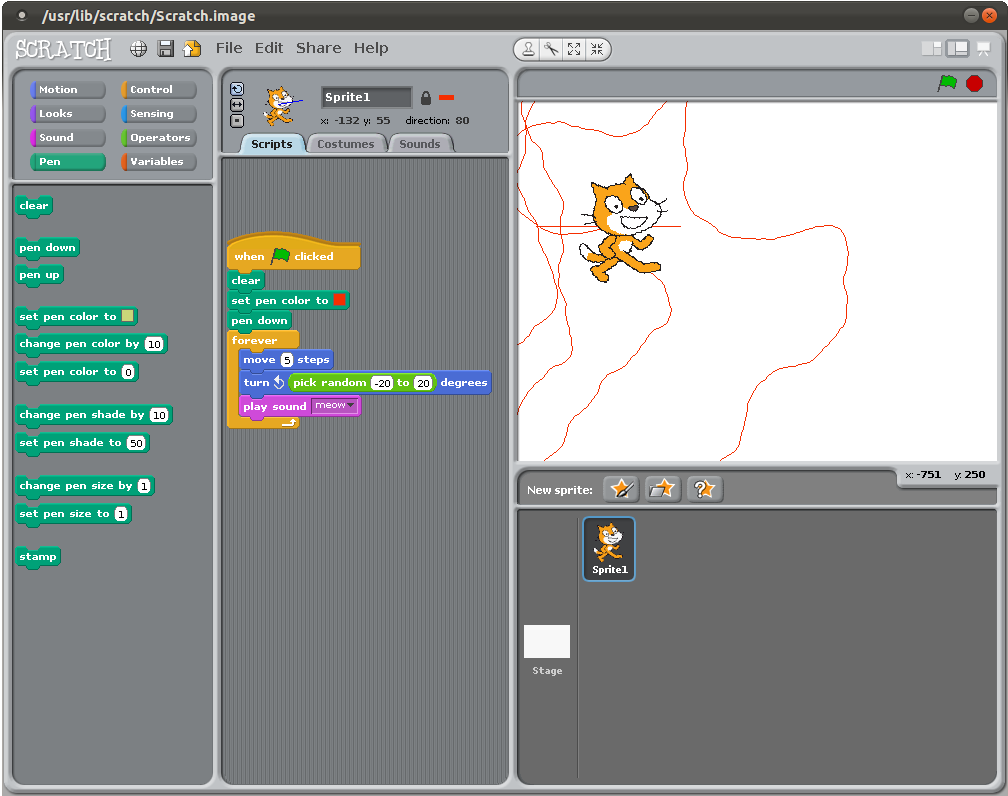
\includegraphics[width = 0.5\columnwidth]{scratch.png}
\caption[The Scratch visual programming language]{A random walk (red line, top right) programmed in the Scratch visual programming language\cite{Resnick09}. Statements are chosen from the palette on the left to be added to the program in the centre. The execution of the program is performed by the cat sprite in a turtle-like manner, top right. Note that invalid expressions may not be programmed, for example there is no attachment point to add a further operation after a ``loop forever'' statement.}
\label{fig:scratch}
\end{figure}

\item We may create graph based graphical visualisations of many aspects of a program. For example the data structures may be modelled by the \emph{Unified Modeling Language} (UML) or we may animate the flow of data\cite{Shizuki00}. These are analytical, not generative, applications of graphs to programming.
%Animating a large program - shizuki et al.
% Typically the visual interface constrains the user to syntactially correct statements.  An early example is PLAY\cite{Tanimoto86}, which allows actions to created by creating linear sequences of pictorial icons . 
\end{itemize}

\FloatBarrier 

As graphical hardware advanced it became clear that the graphical editing of data flow programs was a good candidate for creating geometric programs. To clarify, not only is the program edited graphically, but also creates geometric output. These systems provide a widely used example of PGM without written programs, albeit under another name. 

The Fabrik Programming Environment\cite{Ludolph88} allowed 2D graphics, user interfaces, and their elements, such as scroll bars, to be constructed within a dataflow environment, but suffered from ``poor performance''. Conman\cite{Haeberli88} utilised data flow graphs on more complex graphics hardware to create 3D objects. A user of the system could construct nodes that interact with the user, allowing user interface sliders, 2D curve editors, and arbitrary scripts to create 3D objects.
Later Lovejoy et al. used the Prograph data flow language to control a 2D turtle\cite{Lovejoy92}, and Abram et al. use data flow languages to visualise 3D data\cite{Abram95}.
More recently, data-flow as a programming paradigm has seen use in the graphics literature. For example, the strict hierarchy and lack of side effects in split shape grammars can be modelled as a visual graph\cite{Patow12}. In \cite{Benevs11} a message-passing approach, reminiscent of data-flow programming, is used to connect otherwise disjoint L-systems. 

%The Fabrik Programming Environment\cite{Ludolph88}: bidirectional data flow? Structural data programming (no loops required). Single portion of teh graph to the the output as a user-frame. Used to build a scroll bar. ``poor performance''.

%via prograph
%Condor: Constraint-based dataflow\cite{Kass92} compiles down to optimised c++ with user interface . notes that lots of graphics (paraemteic curfaces, shaders) have few side effects and are deeply parallelisable. contains solver. pull data flow evaluation (lazy eval). Applied to vision (motion capture), 2d and 3d curves/splines.
%An Extended Data-Flow Architecture for Data Analysis and Visualization\cite{Abram95}


%Graphically Defining New Building Blocks in ThingLab \cite{Borning86} (part of chapter 7 415 in big red) Sutherland introduced an early graph editor which utilised a light-pen as an input device\cite{Sutherland66}. Sets of constraints that work in both directions to define programs, graphs and circuits. Works to solve these constraints in a variety of intereseting ways.

Perhaps more significantly, the data flow model is used extensively in recent commercial software; \emph{3D modeling packages} frequently utilise some form of data flow graph as an alternative to scripting languages. Both Alias' Maya's \emph{Hypergraph} and Blender's \emph{Nodes} use data flow graphs to describe causality within complex kinematic systems, and the relationships between different texture channels. OpenDX\cite{Thompson01} uses data flow graphs to allow users to quickly visualise data sets of a wide variety of types, as in Fig~\ref{fig:opendx}. The hierarchical compartmentalisation makes shape grammars a target for data flow graph editors, as implemented in CityEngine\cite{cityEngine}.
A more general dataflow programming system is given by the likes of Generative Components\cite{bentley} or Grasshopper\cite{grasshopper}. 

\begin{figure}
\centering
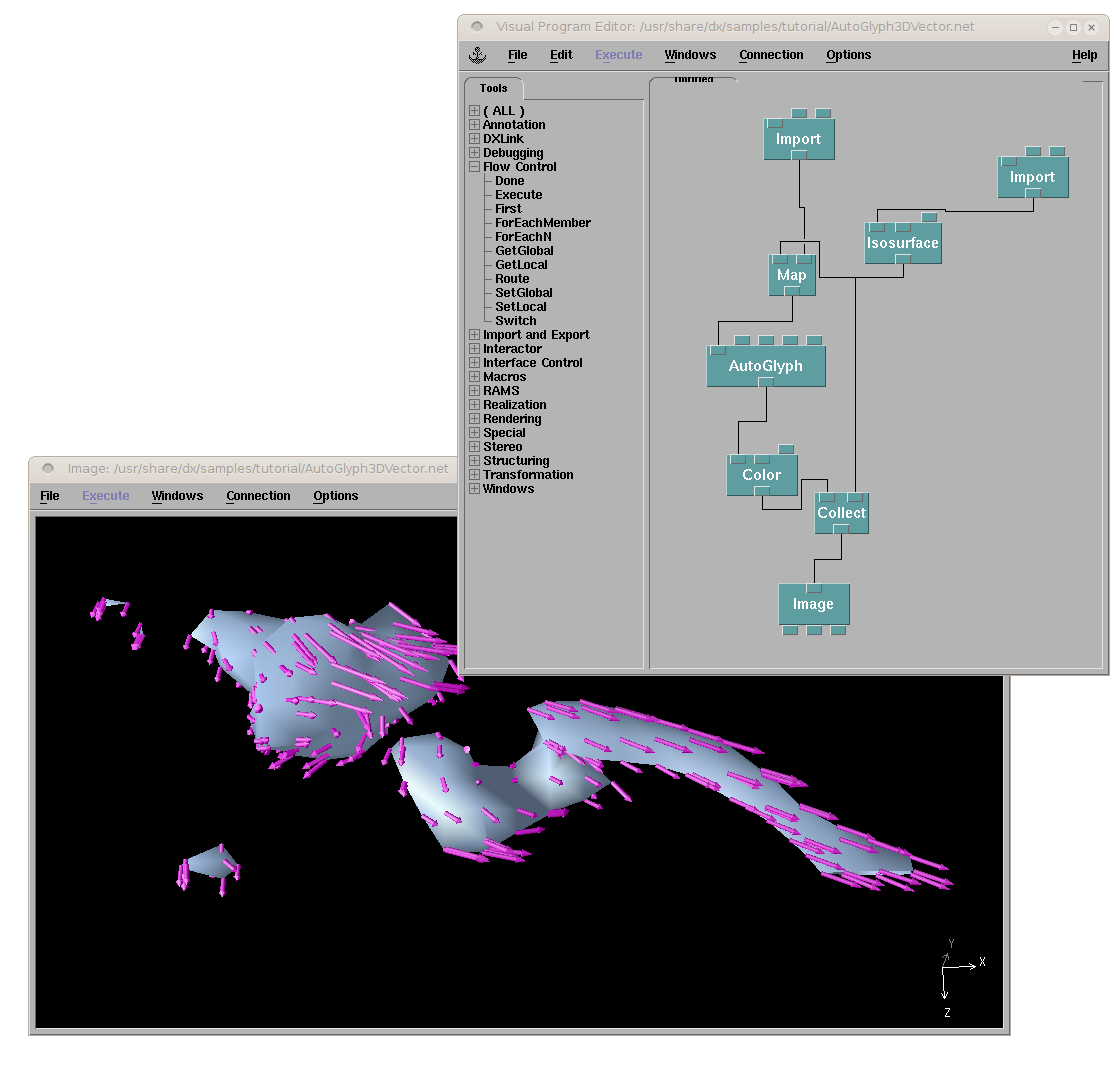
\includegraphics[width = 0.8\columnwidth]{opendx.png}
\caption[The OpenDX visual programming language]{An example of data flow being used to configure the visualisation of a surface via OpenDX. The two paths the data takes through the graph construct the isosurface and surface velocity, before combining them into the single 3D view.}
\label{fig:opendx}
\end{figure}

To conclude this discussion of data flow graphs we introduce details of Grasshopper to give an indication of the typical tools available in these languages. Grasshopper uses a structural data flow graph to describe procedural geometry. We give an example of a Grasshopper data flow graph in Fig~\ref{fig:grasshopperGraph}, to create the geometry of a procedural truss bridge in Fig~\ref{fig:grasshopperResults}.

\begin{figure}
\centering
\def\svgwidth{0.6\columnwidth}
\includesvg{11-readings/images/grasshopperResults}
\caption[Editing the parametrisations of the model in Fig.~\ref{fig:grasshopperGraph}]{\label{fig:grasshopperResults}The result of varying the parameters $v1, v2$ \& $v3$ in the Grasshopper parametric model of Fig.~\ref{fig:grasshopperGraph}.}
\end{figure}

\begin{sidewaysfigure}
\centering
\def\svgwidth{0.9\columnwidth}
\includesvg{11-readings/images/grasshopperGraph}
\caption[A Grasshopper data flow graph]{\label{fig:grasshopperGraph}Top: A graphical geometric data flow graph in Grasshopper. The model is controlled by three numeric parameters $v1, v2 $ \& $v3$, controlling the number of vertical beams, the curve of the arch and the number of horizontal beams respectively. Bottom: The truss structure generated, colour coded to indicate the graph nodes that created the geometry, starting with the grey rectangle input to the system (top, far left).}
\end{sidewaysfigure}

The structures transmitted along the arcs are nested lists, each nested to a depth specified at compile time. Because only lists with the same nesting depth can be used as inputs to the same function, Grasshopper's UI indicates the nesting depth by the type of line between nodes (undecorated, double or dashed lines for single elements, lists-of-elements or lists-of-lists-of-elements respectively), as in Fig~\ref{fig:grasshopperGraph}. To address the sequencing issue, when an operation node takes more than one input Grasshopper specifies several data-matching techniques, demonstrated in Fig.~\ref{fig:dataMatching}, based on the number of evaluations of the operation --- either the shortest, longest, or product of the sizes of the inner most list. In addition there are a number of operations for re-ordering or selecting elements from the data structure, marked by $\ast$ in Fig.~\ref{fig:grasshopperGraph}. However they are only able to manipulate elements in the inner-most list; more complex patterns require writing programs to order the nested lists.

\begin{figure}
\centering
\def\svgwidth{1.0\columnwidth}
\includesvg{11-readings/images/dataMatching}
\caption[Data matching in Grasshopper]{\label{fig:dataMatching}Data matching in Grasshopper. When joining the horizontal truss members, three techniques are offered --- Left to right: \emph{Shortest list}, \emph{longest list} and \emph{cross reference}.}
\end{figure}

As an aside we note that data flow programming in no way alleviates the standard numerical computation issues, as witnessed by the removal of a small delta in two places of the computation, marked \textdaggerdbl\; in Fig.~\ref{fig:grasshopperGraph}.


%%%%% graphical applications of data flow.

%“Conman: A Visual Programming Language for Interactive Graphics,”\cite{Haeberli88}. User defines flow of data between different elements, such as sliders, curve editor, tape storage, renderings and scripts. conman == connection manager. Creates 3d vieweable renderings.
%Guided Procedural Modeling\cite{Benevs11}: connecting procedural systems via links that pass messages. Very much like dataflow. applications to trees, dinosaur shaped bushes and street layouts. 
% more of a constraint solver, like thinglab. Show and Tell: A Visual Programming Language. (page 397 in red book) \cite{Kimura90} Emphasis on not using hte keyboard. Subroutines, iteration recursions and concurrency represented by 2 patterns.designed for school children. Dataflow loops dificult for children. directed acyclic multigraph. . Represents variables as ``completion problems'' - unknowns that will be calculated by the computer to satisfy some conditions. System of boxes for highlighting thrown excpetions while executing pthe program. box is subroutine. If there is only one way of filling boxes without excpetions, then it's a function, else it's search space. Can recursivlely apply boxes for iteration. Notation for repeating boxes, repeats until inconsistent!

%%%%%%%%%
%“Advances in Dataflow Programming Languages,”\cite{Johnston04} Dataflow originally for parallel programming and avoiding von neumann bottlencke. We may execute any operation that has data waiting, rather than just the one at the current program counter. Long list of visual programming languages. Concept of gates as filters for data streams. Arcs in graph are FIFO queues

%pure dataflow works on flowing tokens, however in the structure model each node creates only one data object as output. - permits radmon access of data procuesd and history senisity. All data create must be stored (pure functional!).  tagged-token architecture: uses tokens to keep track of the result values (for a repeatedly invoked sugraph or iteratation). A node waits till it has each input of the same colored token. Pure dataflow, needs to be careful about synchronising inputs, tagged-tokens don't.

%c/p from page 10:
%(1) freedom from side effects,
%(2) locality of effect,
%(3) data dependencies equivalent to scheduling,
%(4) single assignment of variables,
%(5) an unusual notation for iterations due to features 1 and 4,
%(6) lack of history sensitivity in procedures

%== very functional. down to the problems with iteration: recursion special rules. Textual dataflow languages exist. VAL: a textual dataflow languae with multiple return values? Mostly used for hardware language design. The development of Grunch supported the claims of Davis and Keller [1982] that software engineering could be as much a motivation for pursuing graphical dataflow as the pursuit of efficient parallelism. Gakski 82 argues against dataflow (page 12) Describes the issues with iteration that functional programs have. No such thing as a program counter in math-speak.
%%%%%%%%%

%Any other follow-ups from Wouter van Oortmerssen Candidate's PhD: Concurrent tree space transformation in the aardappel programming language?

%http://c2.com/cgi/wiki?GraphicalProgrammingLanguage
%http://www-ist.massey.ac.nz/plyons/776/VPL%20papers.html


%%%% JUNK %%%%%

%Pygmalion: a computer program to model and stimulate creative thought\cite{Smith77}
%The FL-system: a functional L-system for procedural geometric modeling\cite{Marvie05} : as above. not for this sectino.
%The  Logic of Architecture: Design, Computation, and Cognition \cite{Mitchell90} first order logic predicates for architecture Mitchell describes the kind of first order logic predicates that may be used to describe architecture. Throughout this lengthy volume many conflicting approaches for describing architecture in logical form are given. None of these are concise enough to implement and the NP-complete nature of inferring facts from logic problems make this approach a little unrealistic. Mitchell does not combine these different ways of viewing architecture into a single model. State space search over these axioms. fromal grammars (Palladian grammar in particular). Composition of functions is procedural modeling?
% Automata
%Voxel space automata: modeling with stochastic growth processes in voxel space \cite{Greene89} Quad tree for fast branch positioning 
%Graph grammars, a new paradigm for implementing visual languages\cite{Gottler89}


\FloatBarrier 

\section{Simulation Approaches} % creating something from nothing.
\label{s:simulation}
% todo: location in procedural spectrum?

Creating grammars to describe man made objects is somewhat natural, as we are able to encode the design process that a human may go through to create an object. However there are many non-designed artifacts that we may wish to model in a procedural manner, for example terrains, the historical growth of cities or damage to trees and plants. \emph{Simulation} approaches to procedural modeling involve the imitation of observed processes to approximate the interactions within a model, and between the model and its environment.

Simulation is used in a wide variety of ways to create geometry; we have already seen examples of grammars simulating the growth of plants using L-systems\cite{Reffye88} and complex systems via data flow graphs\cite{labview}. We might even consider that searching through grammar derivations is a simulation of the human design process. This section explores a collection of systems that have simulation in common.

A very simple form of simulation are \emph{cellular automata}; a specific example is provided by \emph{Conway's Game of Life}\cite{ConwaysLife} in which every simulation step updates a 2D array of cells (boolean values) using very simple rules. As illustrated in Fig.~\ref{fig:cgol}, these simple rules are executed in parallel on every update step, possibly changing the value of a cell. Despite the simplicity of the rules, different starting values for the cell yields a wide range of persistent and varied forms.

\begin{figure}
\centering
\def\svgwidth{1.\columnwidth}
\includesvg{11-readings/images/cgol}
\caption[Conway's game of Life]{\label{fig:cgol}Left: \emph{Conway's Game of Life}\cite{ConwaysLife} simulation takes place on a 2D grid, the transition from a living (black) to a dead (white) state occurs based on the current state and the eight neighbours (top). Middle: The glider pattern, which self-propagates along a diagonal as the simulation progresses. Right: A space-filling pattern by Hartmut Holzwart, at simulation steps 0, 10 and 200.}
% from golly game of life simulator spacefiller.rle file
\end{figure}

Attempting to program Conway's Game of Life for a particular purpose is often quite involved, however it delights in the unexpected behaviours that may be observed as the simulation progresses. These unexpected or \emph{emergent} behaviours have been better studied in simpler still automata, such as those 1D systems studied by Wolfram\cite{Wolfram03}. Fig.~\ref{fig:rule30} shows certain very simple rules creating complex patterns. There are 256 similar sets of rules, and this example is one of two examples that exhibit these emergent properties, generating aperiodic, non-local structures. 

\begin{figure}
\centering
\def\svgwidth{1.\columnwidth}
\includesvg{11-readings/images/rule30}
\caption[A Wolfram class VI automata]{\label{fig:rule30}A Wolfram cellular automata defines a transition over a 1D sequence of cells who are either alive (black), or dead (white). Left: In this particular case ``rule 30'' specifies these eight transitions given a context of three cells (the cell to the left, the cell itself and the cell to the right). Middle: When applied in parallel these rules mutate a start state consisting of a single black cell in a deterministic manner. Right: We may repeat this procedure a large number of times to generate an complex emergent system of local structures throughout the right hand side of the pyramid.}
\end{figure}

Emergent behaviour seems to be very powerful as it produces intricate patterns from very concise descriptions. For these reasons simulation seems to lie on a cusp on our spectrum of procedural modeling. Those general models that we have already examined, may exhibit emergent behaviour, while those that follow are less likely to. However, by definition, emergent behaviours are not intended. It is difficult to engineer these system with particular properties; perhaps the only way of working with these systems is to have a large library with known behaviours, and to select the system with the most desirable properties. 

Turing's work on emergent patterns in physically based simulations\cite{Turing52} suggests that this library approach may be the one favoured by natural selection; appropriating emergent patterns into situations where they are evolutionary advantageous. However these approaches have not found much traction in the computer graphics and procedural modeling mainstream. Examples are limited to corpora to texture synthesis \cite{Meinhardt87} and the physical simulation of plants. Smith et al. construct a time-based 3D growth simulation of the meristem (growing tip of a plant's shoot) in \cite{Smith06}. By modeling the flow of growth hormone auxin through this region, and the geometric changes that it produces, the model produces a realistic geometry demonstrating several modes of Phyllotaxis.

As well as simulating the processes within a plant, there is also a body of work that simulates the environment surrounding a plant. 3D (\emph{voxel}) cellular automata may be used to model the intersection, proximity and occlusion of a plant\cite{Greene89}. Traumatic events, such as branches breaking may be modeled as step events during the simulated growth of a plant\cite{Reffye88}. The growth of a tree through a volume can be simulated as a space colonisation algorithm\cite{Runions07} while structural simulation can create balanced trees\cite{Hart96}. Finally some systems simulate the interaction between both internal and external factors; for example work by Prusinkiewicz et al. growth\cite{Prusinkiewicz96} simulates both the plant-state, via  L-systems, and exogenous factors such as the availability of daylight and water.
 
%Interaction between L-systems \cite{Hart96}. Predictive tools for those in forest managment as well as graphics. Structural simulation of the mass of each branch to simulate howthe tree balences, photosynthseis return of the leaves to simulate photopism

%Plant models faithful to botanical structure and evelopment\cite{Reffye88}, including damage etc... Growth, ramification and mortality simulated over time. traumatisms: growth model may simulate chance of break or death of the apical (bud at the tip of a growing branch). Somewhat similar to L-systems, but not.

%Visual models of plants interacting with the enviornments in\cite{Prusinkiewicz96}. Attempt at a universal environmental feed back mechanism - now sensitive to self and exterior conditions. Bidirectional information exchange between model and environment. Includes environemental response. 

%Voxel space automata: modeling with stochastic growth processes in voxel space\cite{Greene89} - voxels. Sensitive to moisture or light, no collision.

%Modeling Trees with a Space Colonization Algorithm\cite{Runions07}. Given a volume for tree foliage, and a trunk-starting point, the system colonises the space and adds plant organs etc. Volume is filled with attraction points - models available space; each new branch segment moves towards the nearest attraction point. Terminates when all attraction points have been removed. Generalized cylinders model variable width limbs.


%Computation at the edge of chaos: phase transitions and emergent computation\cite{Langton90}: ``life at the edge of Chaos''. For emergent behaviour, transmission, storage and modification of information must be present.

%Universality and complexity in cellular automata\cite{Wolfram84} Class I evolves to a homogeneous state. Class II evolves to simple separated periodic structures. Class III yields chaotic aperiodic patterns. Class IV yields complex patterns of localized structures.

%Emergent behavours.
% include: \section{Statiscial} % perlin noise, terrains etc..
% reaction-diffusion systems.

%A Chemical Basis for Morphogenesis \cite{Turing52}. The equations that simulate chemical diffusion, and chemical interactions. Stationary wave patterns, suggests that dappling patterns, and stationary waves in 2D could acocunt for phyllotaxis.

%A plausible model of Phyllotaxis.~\ref{Smith06}. Models auxin level, flow and creation and transport between cells. 3D cell simulation results describes the different modes of Phyllotaxis ``frequently observed transition from decussate to spiral phyllotaxis''. Small quantitiy of noise in initial set required to generate patterns.

%unused:
%Towards the systems biology of auxin-transport-mediated patterning\cite{Berleth07}. Auxin generates an axis that severs a location system for subsequent patterning events.

%Modeling and Visualization of Biological Structures\cite{Prusinkiewicz93}. 
%Read section 4.1 in carlos' EG star

%constraints? optimisation?

Another frequently simulated domain are cities. Many systems exist for modeling land use, populations and travel costs within cities\cite{Waddell:2002,Simmonds99}. Mostly these use grids of data points, or fixed-structure cells to represent design and layout, some even use cellular automata to model these processes\cite{Kheder08,Honda04}. 


The introduction of PGM to urban modeling simulations has allowed the creations of detailed visualisations of the resulting cityscapes that change over time. Typically geometric city simulations follow the same procedural urban modeling ``waterfall'' pipeline as time-static procedural cities\cite{Parish01}, an example of which is given in Fig.~\ref{fig:umPipeline}. \emph{Major roads}, such as motorways and A-roads provide access to a \emph{quarter}, an area with particular characteristics. Access within the quarter is provided by \emph{minor} B-roads. The area between B-roads becomes \emph{blocks}, which are further split into \emph{parcels} of land. Finally buildings are positioned on the lots --- the 3D geometry described by \emph{mass models}, each face of which is then assigned a \facade{}. When working with discrete time-step simulations, as in the 2D model by Vanegas et al.\cite{Vanegas09:VOS} or 3D model by Weber et al.\cite{Weber09}, it is necessary to repeat this course to fine hierarchy with every time step. Examples of Weber's resulting land-use and transport map are given in Fig.~\ref{fig:weber4d}. 


\begin{figure}
\centering
\def\svgwidth{1.0\columnwidth}
\includesvg{11-readings/images/umPipeline}
\caption[An urban modeling pipeline]{\label{fig:umPipeline}A typical urban modeling pipeline, similar to \cite{Weber09} and \cite{Vanegas10:MAB}.}
\end{figure}

This concept of a single pipeline is a gross simplification of the processes that occur within a real city, in which many other factors are considered --- for example major roads must take into account and avoid historical buildings. However the waterfall pipeline is a computationally efficient system with proven results.  A system that allows for interactive feedback between users of the simulation and the system itself is presented by Vanegas et al.\cite{Vanegas09:IDU}. The user may edit values in the simulation using a paintbrush tool, after which the simulation then commences and the system brings the underlying behavioural and urban models back into equilibrium under the new assumptions. This is a useful urban planning tool for quickly examining the results of decisions, such as building new roads in neighbourhoods.

\begin{figure}
\centering
\def\svgwidth{1.\columnwidth}
\includesvg{11-readings/images/weber4d}
\caption[Simulating the growth of a city]{\label{fig:weber4d}The work of Weber et al. (\copyright 2009) simulating the geometric growth of a city\cite{Weber09}.}
\end{figure}

A further use for simulation at the building level is for the investigation of the physical strength of a system. For example we may wish to:
\begin{itemize}
\item identify the safe range of parameters in a parametric model, such that our building is able to support itself\cite{Whiting09}.
\item design a truss structures to support certain loads\cite{Smith02}.
\item find self-supporting free-form surfaces\cite{Vouga12} that are sufficiently strong to be constructed.
\item build furniture that is both stable and durable\cite{Umetani12}.
\end{itemize}

Each of these systems allow the user to specify a model and then simulation is used to search for physically stable variation. This approach blends artistic human design elements with automated reasoning about the properties of such a design.

Finally we find systems that use simulation for interior design. Two recent systems attempt to position a given set of furniture in room by maximising an evaluation function. Merrel et al.\cite{Merrell11} encode various interior design guidelines, such as the  distance chairs should be from one another to permit conversation. Starting from a user suggestion, the system is able to find a solution that accommodates these guidelines. Alternately Yu et al.\cite{Yu11} learn pairwise relationships between items of furniture from several examples, and include occlusion constraints to ensure clear paths between doorways. Both of these systems simulate a walk through an evaluation function by \emph{Markov Chain Monte-Carlo} sampling. While this is perhaps not simulation in the classical sense, it may be seen as simulating a human designer's exploration of the design decisions.

%Interactive Furniture Layout Using Interior Design Guidelines\cite{Merrell11}. Given a room, and various objects, how should they be distributed. System creates suggestions. Can select focal point. Density function encode design guidelines explored by a a markov chain monte carlo sampler, and samples drawn via by the metropolis-Hastings algorithm.

%Make it Home: Automatic Optimization of Furniture Arrangement\cite{Yu11}. Same setup: room + furniture. Pairwise relationships between objects, paths between doors, and clearance around objects.  Stochastic optimization with a m-h step, converges over many iterations. Knows about putting things on other things. Relationships learnt via positive examples. 

%Guided Exploration of Physically Valid Shapes for Furniture Design\cite{Umetani12}. Interactive furneture design system that warns and offers corrections if the design in unstable or not durable. Leaves aethetics to users, technical detilas handled by machine. Physical simulation.

%Fuzzy inference guided cellular automata urban-growth modeling using multi-temporal satellite images\cite{Kheder08}
%Generating Autonomous Time-Varying Virtual Cities\cite{Honda04}. Block status determined by automata. Poor paper - details a method of simulating city through time, but lacking many details.
%UrbanSim: Modeling Urban Development for Land Use, Transportation and Environmental Planning\cite{Waddell:2002} Urban model that uses grid cells.

%Visualisation of simulated urban spaces: Inferring parametrised generation of streets, parcels, and aerial imagery.\cite{Vanegas09:VOS}. Visualising simulated cities. Gather stochastic data from a map, then use simulation data to to create a plausible layout. - creating parcels, street etc... Contains parcel-creation techniques.

%Interactive Geometric Simulation of 4D Cities\cite{Weber09}. Integration of detailed geometry into simulation, to allow the geometric growth of realistic cities. (integrates geomtery, street expansion, traffic computation, land use lot subdivision and building envelope. Medium sized cities can be generated interactivlity. Discrete steps of simulation.

%Interactive design of urban spaces using geometrical and behavioural modeling\cite{Vanegas09:IDU} Behavioural (population, jobs accessiblity, land value) and geometric modeling (roads, blcoks, parcels, buildings). Interactive generation times. Agent based behavioral modeling system. Variable editing via paint brush, then the system attempts to bring the urban model back to equilibrium. Demo - sketching a highway spreads the city out.

%Creating models of truss structures with optimisation\cite{Smith02}. Non-linear optimization - repeadly solve a system for geometry (lengths), then remove any short beams. Physically realistic structures, Such as the Eiffel tower. User positions anchors and a set of loads, system positions additional ``free joints'', acording to the bridge type specified by the user. Ban beams in certain obstical areas, allowing user to sculpt the truss.

%Procedural modeling of structurally-sound masonry buildings\cite{Whiting09}. Parameters controllsing features of a grammar are found that lead to stable / structurally sound (and realistic) models. Compute static forces on inter-element boundaries - blocks considered rigid. PArameterised shape grammar. User designated parameters to solve for (eg wall thickness or window width). Iterative downhill search search for a minimum-energy system that is stable. Results show that elements are not repeated more or less, just resized.

%Design of self-supporting surfaces\cite{Vouga12} Given a surface, propose a similar surface that is self-supporting. Self supporting means that you could build it from masonry, with motar/friction holding it together (inf compressive strength). Models the stresses as a thrust network. Manifold surfaces only.

%not used Procedural generation of roads\cite{Galin10}. Shortest path, weighted by hills, obstacles etc.. attempting to simulate the design process? Mimize cost function.  A star shortest path. Excavates terrain to fit. cust functions for curvature, water depth, slope, tunnel cost. 

% cheapest?
%Not simulation based:
%The automated generation of architectural form \cite{Mitchell71} search space for simple toys, introduces for buildings. very philosphical, early work.
% Mention crowd simulation?

\section{Inverse Procedural Modeling}
\label{sec:inverse}

As we have seen, the creation of procedural models is quite involved, requiring considerable knowledge of grammars and languages. Recently there have been attempts to generate procedural models from real world examples, the process of \emph{inverse procedural modeling}. As with much of the shape grammar literature, the focus has been on applications to the urban environment.

The data from the input examples may have been captured via multiple cameras and terrestrial or aerial LiDAR (LIght Detection And Ranging, Sec.~\ref{sec:construction} contains further details); therefore it may contain significant quantities of noise. Identifying features in this data is the first challenge, for urban environments in particular repeated features are of significant importance. Recent techniques\cite{Mitra06,Pauly08} for identifying such features in noisy data cluster the transforms between similar local features to determine prevalent transforms. To reduce noise in the input data, RANSAC\cite{Fischler81} is a popular algorithm, and is utilised by GlobFit\cite{Li11} to clean meshes making assumptions about features such as planar surfaces, repeated distances and shared angles. Finally we can form descriptions of 3D meshes as a tree of such patterns and symmetries\cite{Wang11} for compression and error correction.

% analysis techniques

%Identifying features in input data is one of the first challenges in inverse procedural modeling. When studing urban envrionments.

%Partial and Approximate Symmetry Detection for 3D Geometry\cite{Mitra06}. Compression of geometry by finding all repeated elements under various transforms. Build shape sig. over local features and cluster. Most likely features under transforms give major symmetries.

%Discovering structural regularity in 3D geometry\cite{Pauly08} sym extraction, using repeating features in a lattice. Used to pull all the repeated elements ouf a facade/point cloud. Reconstruction of collosium

%GlobFit: consistently fitting primitives by discovering global relations\cite{Li11} Finds copplanar faces, matching angles, edges of equal length in manmade structures usign RANSAC. Recovers these from noisy data: point clouds, identifying shared patterns.

%Symmetry Hierarchy of Man-Made Objects\cite{Wang11}. 3Dmodel -> segment -> hierarchy of parts via found symmeteries.

% todo cite the review paper by musialski

%%%

The grammar extraction techniques presented in this section mainly use the models derived to compress data, rectify noisy captured data, or to extrapolate data to fill holes. There has been relatively little work to re-target the extracted procedural models to create novel geometry.

Before we examine systems that derive entire grammars themselves, we note that there is a quantity of work on fitting parametric models to existing data. In the field of urban layout reconstruction Aliaga et al.\cite{Aliaga08} learn descriptive parameters for a road network via statistical analysis; this is then used to create new road maps. Alternatively a template shape grammar may be parameterised to match input from vision techniques\cite{Mathias11}.

%%%

The construction of grammars from examples has proved difficult, and the majority of solutions rely on meta-heuristic techniques to search for a suitable candidate. Typically these techniques repeatedly manipulate the grammar and compare the current results with the noisy input data. In early work, Dick et al.\cite{Dick04} fit a grammar from several images using a \emph{reversible jump Markov chain Monte-Carlo} technique. The grammar used is relatively simple --- a set of walls formed the model, and each wall having a set of associated decorations. The work is notable as it was able to reconstruct unseen portions of buildings. Another system that uses a simple grammar and rjMCMC is that of Ripperda et al.\cite{Ripperda08,Ripperda09} who utilise \emph{minimum description length} of the derived grammar as an evaluation criteria. By simplifying the grammar to an assignment of a parameterised mass model to a number of quads covering the floor plan, \cite{Lafarge10} successfully used rjMCMC to reconstruct large cities from aerial data.

More generally, rjMCMC has been recently used to force the derivation of an arbitrary stochastic context free grammars to posses some specific qualities\cite{Talton11}; for example the silhouette of a derived tree to some specified shape.

An alternative meta-heuristic for creating grammars are evolutionary algorithms. Simon et al.\cite{Simon12} exploit a \emph{Pareto} evolutionary algorithm to evolve a \facade{} shape grammar matching a number of images. In this system the appearance from multiple views, and the depth correspondence form the evaluation (evolutionary fitness) function. 

An incidental generation of grammars occurs in several places in the urban reconstruction literature. As \cite{Han:2005:BTI} and \cite{Becker09} typify, the grammar complements the bottom-up landmark cluster analysis with a top-down grammatical description of the scene, enhancing feature extraction. An alternative approach\cite{Toshev10} is to only apply the bottom-up clustering analysis, using the grammar to describe the properties derived from the input data.

%Modelling and interpretation of Architecture from Several Images. rjmkmc to explore geometry space.\cite{Dick04} 2-6 images as input. Produces labelled outptu. Prior model from training data and architectural experts. Explored using rjmcmc. Model is a set of walls, and associated decorations. Can model hidden parts of the building via the grammar. textured result. 

%Bottom-up/top-down image parsing by attribute graph grammar. \cite{Han:2005:BTI}. Good work! Attribute graph grammar for parsing scenes made up of rectangles. Bottom up rectangle detectection with top-down preditction via the grammar. Many rectangles noisily detected to begin with - use the grammar to connect all rectangles that we output. Eg: poorly rated rectnagles, have their weights increased if supported by a gramamr rule.

%Determination of facade attributes for facade reconstruction\cite{Ripperda08}\cite{Ripperda09}.  Poor paper. Reversible jump markov chain monte carlo for reconstructing facades grammars from images. Similar to: Application of a formal grammar to facade reconstruction in semiautomatic and automatic environments.\cite{Ripperda09} . MDL to guide likelyhood of facade model being correct. more rjMCMC. Discusses ambiguoity - which is the right grammar.

%Generation and application of rules for quality dependent \facade{} reconstruction\cite{Becker09}. Top down and bottom up strategies. LiDAR input. Grammar fills in missing data. Find terminals via split to floors, then each floor into tiles via vertical features. fills in missing parts, can infer missing parts between buildings.

%Detecting and parsing architecture at city scale from range data.\cite{Toshev10}. Builds a tree of volumetric parts, based on adjacencies. Input is point data. One main root node. Leaves are non-vertical planar patches (roofs + misc). RANSAC to pull planes from clouds. Builds a grammar by applying heuristics to these terminal patches and volumes.

%Structural approach for building reconstruction from a single DSM\cite{Lafarge10}. More rjmcmc. Automatic or Interactive exctraction (eg positions triangles and quads). 2D supports are plans that are assigned one of several parameterized buildings+block-roofs, minimised energy to ensure that the blocks can be put together.

%Metropolis Procedural Modeling\cite{Talton11}. Given a parametric stochastic conditional context free grammar grammar, compute a derrivation in that grammar that fufills certain properties. Sampled reversible jump Markov chain Monte Carlo explortation of the fitness function optimization.

%Parameter-free/Pareto-driven Procedural 3D Reconstruction of Buildings from Ground-Level Sequences\cite{Simon12}: reconstruction of grammars from 3d point clouds taken from photographs. Evolutionary algorithm to fit a shape grammar.

%Image based procedural modeling of facades\cite{Mueller:2007:IBP}. Mutual information to identify similar, repeated facade tiles or floors. Can then build a split-grammar using a shared hierarchy over repeated componeents. Then 3d elements are matched and a CGA Shape grammar extracted.

% learning parameters

%Procedural 3D Building Reconstruction using Shape Grammars and Detectors\cite{Mathias11}. Template shape grammars, tuned by point cloud data: they find the parameters. For example different temples... Feedback from grammar fit to update vision subsystem. Online service for photo-> point cloud. Ransac for plane fitting. Identifies repeats.

%Interactive example-based urban layout synthesis\cite{Aliaga08}  Vector and image based synthesis. Tree-structure of vector and bitmap data. Interactive approach. Sythesis of streets by statistics. Parcel allotment via bounding box, dividing line, random point placement + vornoi. Image synthesis by quad-morphing. Users select type of join, blends between layouts.

%%

To avoid the need for meta-heuristics entirely M\"{u}ller et al.\cite{Mueller:2007:IBP} use the concept of mutual information to identify repeating patterns in images of \facades{}. The presence of strong horizontal or vertical lines is used to determine the split-locations to generate a CGA Shape grammar. This leads to a compact representation of the \facade{} that can be manually extrapolated to 3D. Another assumption that simplifies the construction of grammars is that of a Manhattan World\cite{Vanegas10}, in which all objects are orthogonal polyhedra.

%Building Reconstruction using Manhattan-World Grammars\cite{Vanegas10}. Assumptions about face directions allow reconstruction or rectlinear buildings using one 2-4 photographs. Not really a parametric model, only reconstruction?


%Inverse Procedural Modeling by Automatic Generation of L-systems\cite{Vstava10}. Reverse engineering of 2D vector forms to L-systems that can then be retargetted/modified by changing terminals etc... Similar elements are assigned terminal symbols. Sequences of terminals identified. Avoids complexity of having to write l-systems. Uses Mitra/06's techniques, clustering transforms to find patterns. Single tree of merges to generate all reules. no grackgracking or real search. 

M\"{u}ller's automated extraction of \facades{} is one example of using the extracted grammars to re-target content. In this case the resulting \facade{} could be re-sized arbitrarily. Another example is \emph{Style Grammars}\cite{Aliaga07}; a building grammar is created from 3D geometry, such that it may be retargetted to a different floorplan or height. This system works principally by analysing the 1D patterns of sequences within a shape-grammar like environment to predict a split rule for the resulting grammar.
Finally Vstava et al. extract L-systems from 2D vector designs by identifying similar components and then analysing the transforms between them\cite{Vstava10}. These L-systems may then be edited to create unique new designs.

Inverse procedural modeling has the potential to create models that may be retargetted to model novel situations, such as constructing buildings of different heights or floor plans. However the results are, by design, derivative of the examples provided. For this reason we may consider inverse procedural techniques to be more specific than general purpose or simulation systems, yet more general than geometry capture or modeling systems. 


%todo: problems with the inverse procedural approach? too automated no choices? no real world examples of grammarizable buildings?  too manual?

%Style Grammars for Interactive Visualization of Architecture\cite{Aliaga07}. Interactive system for the creation or modification of existing builings. Extracts grammar, and retargets to new model. 3D Model -> grammar. Assumptions that model is first floor, intermediate floors, roof. Each floor == row of columns. Can recover 3d from 2d image. Stylisation rendering too.

%However the extraction of grammars is the first step in attempts to retarget a grammar to different situation\cite{Aliaga07}.

%passed on: 
%Extracting buildings from aerial images using hierarchical aggregation in 2d and 3d.
%Semi-supervised incremental learning of hierarchical appearance models.\cite{Wenzel08}
%Single view reconstruction using shape grammars for urban environments. 
%Implicit shape models, self-diagnosis, and model selection for 3D façade interpretation
%Interactive 3D building modeling using a hierarchical representation. not really a grammar - just lod data capture.
%Guided procedural modeling\cite{Benevs11}: message parsing between discrete grammars to allow different grammars to fill different volumes, yet still communicate.
%manual
%A GML shape grammar for semantically enriched 3D building models\cite{Hohmann10}. Addresses the problem of editing virtual buildings once they've been created - ``what if a measurement was wrong in the original?''. Manually writing rectlinear split grammars in GML, and demonstrating how we can edit them later.
%CityFit: High-quality urban reconstructions by fitting shape grammars to images and derived textured point clouds\cite{Hohmann09}. Acquistion via LiDAR + multiple cameras, to include annotations. Deconstruction to shape grammars as compact representations of geometry, which also support multiple levels of details. Subcomponents manually marked up (for now!). Start with one of several grammar templates. Shape grammar inside GML. No method for automated grammar extraction!



\section{Combinatory Modeling} 

A subset of the inverse procedural modeling techniques that have an emphasis on usability are \emph{combinatory modeling} techniques.  Combinatory modeling assembles subcomponents of example objects to create unique new geometries. These techniques fall into one of three broad categories based on the level of input that the user is required to supply. % do we highlight these three levels?

Combinatory modeling obtains its procedural element from the choices made during automated assembly. When there is a choice of the choice of parts to attach, a range of designs may result. However, whatever algorithm is used to make the derivation choice, the result can only comprise subcomponents of the examples. For this reason combinatory modeling is a very domain specific technique in our procedural spectrum.

Early work in combinatory modeling  was inspired by the 2D case of synthesising textures. Given an example texture in the form of a bitmap, \emph{texture synthesis} aims to generate additional bitmaps that are at the same time characteristically similar to the input and yet unique. As in Fig.~\ref{fig:tSynth}, the standard technique is to grow an image from an example texture by combining pixels from the example in a novel order, based on their neighbourhood. To synthesise a certain pixel adjoining the patch, local pixels from the patch form a feature vector. This is compared against all possible vectors in the example texture to find the best match\cite{Efros99,Wei:2000:FTS}. 

\begin{figure}
\centering
\def\svgwidth{1.0\columnwidth}
\includesvg{11-readings/images/tSynth}
\caption[Texture Synthesis]{\label{fig:tSynth}Texture synthesis by the method of Wei et al.\cite{Wei:2000:FTS}. Left: An example tree bark texture. Middle: The results of the synthesis. Synthesising a pyramid of textures helps preserve large features. Right: Each pixel in a scan-line ordering of the new texture is synthesised in turn. The feature vector of the red pixel is shown in the bottom right, This will be compared to the example texture to identify a suitable colour for the pixel.}
\end{figure}

Variations of texture synthesis include \emph{image quilting}\cite{Efros:2001:IQF}, which creates a reasonably coherent grid of overlapping square texture tiles from the example texture. A minimum error cut then determines the exact boundary through the overlapping pixels. An alternative approach is to ensure that the tiles are always positioned in such a way that adjacent borders do not contain discontinuities. An example of this approach is Wang tiles\cite{Cohen03}.

When attempting the synthesis of 3D mesh-based geometry, local features, such as those in texture synthesis, have been successful in reconstructing small missing patches of meshes\cite{Sharf04} using iterative refinement of nearest neighbour search and blending techniques. The synthesis of entire objects has been attempted by tiling 3 space with compatible cuboids, with early examples using \emph{Wang Cubes}\cite{Sibley04}. Later examples by Merrell et al.\cite{Merrell07} use learnt adjacencies between neighbouring cuboids. Merrell extended his work to arbitrary meshes\cite{Merrell08}, from which common adjacencies are extracted, and a backtracking search constructs a new model consistent with these adjacencies. The system is able to create a large quantity of architectural models with only a single mesh as input, and no further user interactions. However the work with tiling geometry retains the limitation that only transformations allowed by the tiling, rather than arbitrary transforms, are present in the output.

Domain specific tools use specialised techniques to relax this limitation and consider non-local portions of the geometry when combining portions of meshes. 
Two notable examples by Aliaga et al. synthesise city layouts, and 
\facades{}. The first system\cite{Aliaga07} extracts statistics about the roads and parcels in an example city layout and and uses them to synthesise new portions of a city. The gaps between the roads are filled with textured parcels generated using a Voronoi tessellation; the textures for these parcels are taken from similar shapes from the example, and morphed to fit. Given a segmented 3D \facade{} the second system\cite{Aliaga07} decomposes it into a simple split grammar by identifying 1D patterns, which can be retargetted to new geometry or floor plans. More recently work has taken place to allow ``intertwined'' 1D sequences of elements over such a \facade{}, allowing for more irregular elements to be represented in a retargettable fashion\cite{Lin11}.

To overcome tiling limitations general symmetry analysis techniques have been developed~\cite{Mitra06} to identify compatible (symmetrical) subcomponents and valid location sites, from an example model\cite{Bokeloh10}. To address the subsequent issue of controlling which of several subcomponents is positioned at a certain site, systems such as those by Kalogerakis et al. introduce a probability based approach\cite{Kalogerakis12} which learns the conditional probability of certain classes of geometry being adjacent, and the spacial relationship between the parts. To gather these probabilities, a large number of examples with subcomponents are required, but the result is a realistic combination of those subcomponents. For example when working with a corpus of aeroplanes, propellers are not combined with jet-engined chassis. 

In contrast to these unsupervised combinatory modeling techniques, \emph{interactive} combinatory modeling of arbitrary meshes is addressed by Funkhouser et al.\cite{Funkhouser04}. This work introduces a tool-chain to allow the user to quickly create detailed models using subcomponents from existing libraries. A shape-based search finds components in a database, and both positioning and mesh blending tools are provided to the user to align and attach those subcomponents to the existing model. This work is later extended to search for 2D sketched profiles of shapes in a library\cite{Lee08}. Other systems specialise in the interactive synthesis by example of repeating 1D systems\cite{Owada06} and the use of genetic programming to inspire the exploration of subcomponent-space\cite{Xu12}.

An obvious limitation of combinatory approaches is that they are only capable of imitating local and global patterns that have already been observed.  While these systems are very successful in combining geometry in new and interesting ways, they are also limited by various geometric cases, where geometric continuity is required between the subcomponents, as demonstrated in Fig.~\ref{fig:combinErrors}.

\begin{figure}
\centering
\def\svgwidth{0.7\columnwidth}
\includesvg{11-readings/images/combinErrors}
\caption[Issues with combinatory Modeling]{\label{fig:combinErrors}Two geometry errors with combinatory modeling systems. Left: From \cite{Kalogerakis12}, the rigging of this novel boat is not attached to the deck because there is no mechanism to deform subcomponents. Right: From \cite{Lin11}, if subcomponents are not carefully selected it is easy for the large scale geometry to contain undesirable patterns, such as the roof on this model of the Parthenon Images \copyright their respective authors.}
\end{figure}

% (pic?! - lin et al's and aliga's morphing failures? and \cite{Kalogerakis12}). furneture setup ignores this entirely.

%A connection between partial symmetry and inverse procedural modeling \cite{Bokeloh10} (todo: to combinatory). Given a model, find symmetrical points using ridgid matching, and use these locations as compatible locations for cut/paste operations . Demonstrated on a castle. build a conetxt free shape grammar from the docking sites and dockers. Possible self-intersection or non-completion when building models. Extension to frid-based geometry.

%Interactive Furniture Layout Using Interior Design Guidelines\cite{Merrell11}. Given a room, and various objects, how should they be distributed. System creates suggestions. Can select focal point. Density function encode design guidelines explored by a a markov chain monte carlo sampler, and samples drawn via by the metropolis-Hastings algorithm.

%Make it Home: Automatic Optimization of Furniture Arrangement\cite{Yu11}. Same setup: room + furniture. Pairwise relationships between objects, paths between doors, and clearance around objects.  Stochastic optimization with a m-h step, converges over many iterations. Knows about putting things on other things. Relationships learnt via positive examples. 

%A Probabilistic Model for Component Based Shape Synthesis \cite{Kalogerakis12}. A statistical model for assembling objects from their component parts. Able to infer how things should be put together using a baysean tree. Statisticaly likelyhood calculated from examples. Runs on cut-up model parts. Can't join cut up parts back together nicely.

%Fit and Diverse: Set Evolution for Inspiring 3D Shape Galleries\cite{Xu12}. Genetic algoritm with part warping/part replacement mutators approach. fitness: ability to stand up. user guided can pick faourites

%Sketch-Based Search and Composition of 3D Models\cite{Lee08}. Extends funhouser04, with better 2d sketch queries to find objects.

%Copy-paste synthesis of 3d geometry with repetitive patterns. Lecture Notes in Computer Science \cite{Owada06}. Simple repeating of a fixed pattern along a path. posts in a fence, floors on a building. Copy, analyse and paste-along-a-1d-path.

%SnapPaste: an interactive technique for easy mesh composition.\cite{Sharf06}. Combining objects - solves for positioning and blending simultaneously. Interactive positioning and blending.


%Interactive example-based urban layout synthesis\cite{Aliaga08}  (move to by example?) Vector and image based synthesis. Tree-structure of vector and bitmap data. Interactive approach. Sythesis of streets by statistics. Parcel allotment via bounding box, dividing line, random point placement + vornoi. Image synthesis by quad-morphing. Users select type of join, blends between layouts.

%Style Grammars for Interactive Visualization of Architecture\cite{Aliaga07}. Interactive system for the creation or modification of existing builings. Extracts grammar, and retargets to new model. 3D Model -> grammar. Assumptions that model is first floor, intermediate floors, roof. Each floor == row of columns. Can recover 3d from 2d image. Stylisation rendering too.

%Structure-Preserving Retargeting of Irregular 3D Architecture\cite{Lin11}. Automating the control of which sections of a model to combine, Lin et al. give us a system to rearrange geometry. Inverse procedural modeling to determine how to fit stuff together. Decome a building's mesh into parts. Interactive resizing. break down a facade into several 1D sequences, which can be retargetted in turn - priamy sequence is longest, others fill in the gaps. User defines boxes, and how things should repeat/scale/stay fixed. Hierarchy of levels of scalings given by yser.. Relies on good initila user partitioning. Mostly box-shaped examples (wouldn't work on roofs?)


%In order to combine different portions of a mesh, similar areas of different meshes must be identified. The portion of this process that has had the most attenting is the identification of regions of meshes that are suitable anchor locations. These may be seams, or elements that are repeated.

%Modeling by Example \cite{Funkhouser04}. Pipeline for user construction of composite models via shape-based search, intelligent scissors, automated positioning, hole cutting and smooth blending. Nice seam-finding (Scissors). Searching via keywords and shape-based search (arm in this position).

%Example-based model synthesis\cite{Merrell07}. Field though up my merrell. Extends 2D texture synthesis to 3D. Profve example model. like 2d, except searches for conflict (space itnersection before intersection). Avoids programming entirely - just create something with matching parts. Ah model is constructed from parts, positioning of parts learnt from model. Lattice based - one item per latti. Search for items we can put next to each other (that do not violate any rules).

%Continuous model synthesis\cite{Merrell08}. Exploits boundary features. Similar connected features. Single model input. ``closed polyhedral object'' as input. based on normal direction. Matches micro, not macro features. backtracking serach of faces, verticies and edges (ident on direction and identitity), just forward assignment of possible edges. Like the 07 paper, but automatic. High complexity to make it work for curves or highly tesslated models.

% not used:
%Graphical search and replace\cite{Kurlander88} early example of shape matching via giving a single example, together with a replacement. UI driven.

\section{Shape Deformation}

% comment on spectrum in simulation - can create a wide range of results with little input within it's domain (eg urban, etc). When used interactively can often suggest a range of possible responses, all of which are desirable/valid within the domain.

% Problems - emergent results can be unwanted, can only work within domain, models are normally trained to 

% easy to use, result is almost always correct. But cannot change structure, often not even add repeats to model. Requires model to exist in the first place.

Moving towards more specific procedural modeling techniques we may decide to only manipulate existing geometry, rather than attempting to design geometry from  first principles . \emph{Shape deformation} is the continuous manipulation of an existing geometry. Typically these models create a range of designs as they deform a shape, and so are a more general procedural tool than geometry construction techniques.

Recent work has begun to explore the overlap between combinatory and shape deformation techniques. Bokeloh et al. continued their work on identifying symmetry\cite{Bokeloh09} to exploit these repetitions to deform models, typically architectural, that contain duplicated elements. These repeats are often reminiscent of combinatory modeling techniques. For example \cite{Bokeloh10} resizes a repeating 1D sequence by repeating symmetrical elements, either chosen randomly, or by a user. An alternative interface is given in \cite{Bokeloh11} which introduces \emph{sliding dockers} as user positionable handles to deform meshes with repeating elements. An underlying elastic deformation is combined with constraints to preserve observed symmetries, such as straight lines or 1D repeating patterns. The most recent system in Bekeloh's series of papers \cite{Bokeloh12} uses a linear system to maintain basic relationships, after factoring out 1D or 2D repeating elements.

%A connection between partial symmetry and inverse procedural modeling \cite{Bokeloh10} (todo: to combinatory). Given a model, find symmetrical points using ridgid matching, and use these locations as compatible locations for cut/paste operations . Demonstrated on a castle. build a conetxt free shape grammar from the docking sites and dockers. Possible self-intersection or non-completion when building models. Extension to frid-based geometry.

%Pattern-aware shape deformation using sliding dockers\cite{Bokeloh11} place arb handles on mesh. Regular and discrete (repeating) properties of mesh preserved. Sliding dockers are 1D patterns that can be repeated within some section of the geometry. Regular patterns found in shape preprocessing, built into sliding dockers. Elastic deformation as base, local constraints to preseve discrete and continuous symmeteres (patterns). More local than the above docking sites, not requiring an entire segement of the model to be edited. Not robust to peturbs in input geometry - messes up pattern recg. Resolving constraints between patterns with different sequences still an issue..

% after above!:
%An Algebraic Model for Parameterized Shape Editing\cite{Bokeloh12} Decomposition into a linear system that can be controlled by a small number of parameters. Repeating patters are factored out, before linear system is created. Nice results on roofs etc, but depends on linear-ness.


% 2 morphing cites (and an image?), then 

The first 2D image \emph{warping} method was created by D. Smythe for the movie \emph{Willow}\cite{Smythe90} in 1988; it was used to smoothly deform a goat into an ostrich, and finally a tortoise. The user specifies the location of key points between the images by positioning a grid, and the system would create an image at a certain interval between the examples, allowing the features to flow to different locations smoothly. To achieve this effect the grid was smoothly interpolated between the two states, and the content of the meshes blended. A similar technique was presented in 1992\cite{Beier92}, that used discrete handles instead of a grid, that weighs each pixel's location relative to each handle. An example is given in Fig.~\ref{fig:morph}. A recent system by Igarashi et al. has a different goal; to allow an image to be deformed as rigidly as possible\cite{Igarashi05}. This is applied to examples to allow the interactive animation of images. A pair of linear solvers allow a mesh to retain a physical rigidity, while being retargetted to a new shape. 
An alternative image deformation technique is image resizing. \emph{Seam carving} is a 2D technique to resize images, whilst retaining the most important features\cite{Avidan07}. By discarding low-energy seams from an image, the most interesting features of an image can be retained, at the cost of global distortions.

\begin{figure}
  \centering
  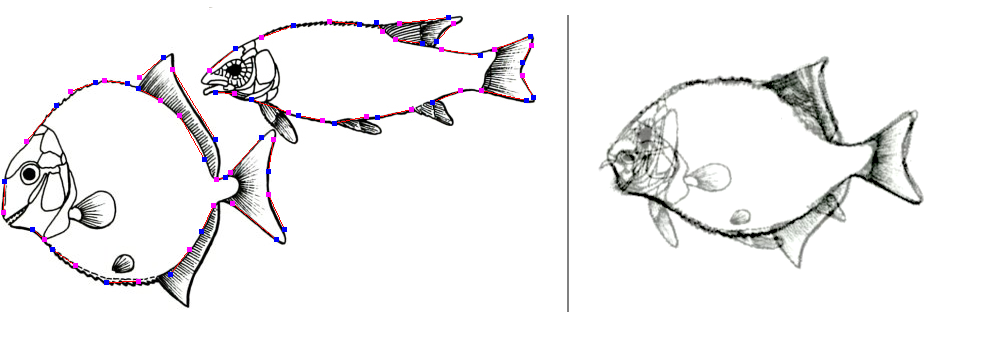
\includegraphics[width=10cm]{morph.png}
  \caption[Image warping]{An example of the `morphing system of Beier and Neely\cite{Beier92}. Left: Two images (black) and their control points (pink, blue). Right: The result of a 50\% warp between the two.}
  \label{fig:morph}
\end{figure}

%todo: Recent Advances in Mesh Morphing 2006 review, m. alexa again

%Seam Carving for Content-Aware Image resizing\cite{Avidan07}. Minimum energy function in two dimensions to resize and image. remove seams with the lowest energy in each direction. Dynamic programming to order the seams.

%As-Rigid-As-Possible Shape Manipulation\cite{Igarashi05}. Interactive 2D system for manipulating images (via triangle  meshes). No skeletal structure given. Depth adjustment so 2D models don't self-intersect. Weights make a portion of the grid more rigid.  touch screen for performance animatin of built models, each point following a finger. USer can position handles wherever. Solved by two least-squares solvers - first for rotation, then for scale.

One of the earliest system to deform 3D objects was created by Sederberg\cite{Sederberg86}. This scheme, analogous to the 2D system of Smithe, utilises a 3D lattice positioned over the object to be deformed. By moving the points of this lattice, the geometry within can be smoothly reshaped without introducing discontinuities. This technique is global, in that the entire mesh is deformed when a lattice point is manipulated. Another global technique\cite{Borrel91} allows the user to position handles on the 3D mesh. After moving these to a new location the system deforms the mesh such that it again touches the handles.

One issue with global deformations is that it is difficult for two physically local sections of geometry to have different deformations without interference. For example, when deforming the middle finger of a hand, it is likely that the index finger will also be repositioned. A response to this was a local deformation --- \emph{skeleton based} deformation techniques, in which portions of a 3D mesh are deformed in response to only a subset of the skeleton. Different portions of the mesh are associated with different portions of the skeleton, allowing for nearby verticies to be manipulated by entirely different deformations. There are many different methods for defining a skeleton ---
\begin{itemize}
\item In early work\cite{Lewis00} the bones that comprise the skeleton are coordinate frames defined by the user.
\item Later systems\cite{Bloomenthal02,Yoshizawa07} use the medial axis of the mesh to define a skeleton as a ``shrunk'' version of the mesh that can be animated and reconstructed.   
\item Lastly we may analyse a mesh to discover mechanical joints, and the joint limits that may be present\cite{Xu09}, to associate the correct portions of the skeleton with the mesh.
\end{itemize}

One issue that is common to most deformation techniques, but skeleton based deformation in particular, is the undesirable self-intersection of the mesh under aggressive editing. Various approaches have been suggested to address this issue, including changing the weights near a sharp bend in the skeleton\cite{Lewis00}, or deforming the mesh based on self-proximity\cite{Yoshizawa07}.

%Pose Space Deformation: A Unified Approach to Shape Interpolation and Skeleton-Driven Deformation% high cite count -- states the the skeleton skinning approach isn't really known, cites maya and some magazine.

%Free-form skeleton-driven mesh deformations%?

%Medial-based vertex deformation\cite{Bloomenthal02} medial axis based deformation - to avoid the problem of global deform fields, use a skeleton - shrink down to a medial axis skeleton and deform that. Weigh edges relitively around juctions to stom self intersections

%Skeleton-based Variational Mesh Deformations\cite{Yoshizawa07}.Automatically derrive the skeleteon from an outline mesh (found via medial axim/ ``blum'' skeleton. Use existing techniques to deform the skeleton, then reconstruct the surface. Use this growth method to avoid self interesction when reinflating skeleton.

%Joint-aware manipulation of deformable models\cite{Xu09}. Allows for deformation using a mixture of rigid components, hinges, and deformable components. Iterative gauss-newton solver is ued to solve the resulting on-linear optimization. Slippable motion analysis to identify joints and joint types (ball and socket, hinge, slippable etc...). Analysis to determine range of freedom for each joint before self intersection. Joint types can be maually asisgned.

%Free-form deformation of solid geometric models\cite{Sederberg86}. Introduce a lattice that lies over the shape (planes, quadrics, parametric surface patchs) in question, lattice can then be used to deform the boundary of the shape. The deformation is specified by berstein polynomials using the control points of the lattice as parameters. Can give continuity control to different degrees (c0, c1...) by position the points at the edge of the lattice clearly.

Both the local and global techniques examined so far have been unable to identify and preserve the symmetries and patterns present in man-made objects. To this end, there have been several recent efforts to create tools specifically targeted to the deformation of man-made objects. For example Cabral et al.\cite{Cabral09} resize meshes using constraints that specify that the angles must remain constant, and the edge lengths must remain as similar to the original as possible. These linear systems can then be solved at interactive rates to allow urban geometry to be resized by a number of user-placed handles. iWires\cite{Gal09} instead analyse the geometry of the given object, to extract a number of wire-like handles that can be used to deform the object. The analysis reveals the symmetries between the wires visible in the shape, and these may then be retained under user edits. Given a model that has a number of constraints, such as orthogonality or planarity, Habbecke et al\cite{Habbecke12} present a method for deformation when the user drags an arbitrary vertex. A combination of a linear model and \emph{compressed sensing} are used to ensure as few verticies as possible are moved.

Some mesh representations, such as \emph{planar quad} (\emph{PQ}) meshes, have underlying constraints on the location of verticies. PQ meshes require that all the faces of a mesh are planar quads, and are useful when, for example, we wish to build curved glass roofs from a patchwork of planar tiles. Yang et al\cite{Yang11} introduce a framework for deforming such meshes by exploring a high dimensional space. This space is bounded by the given constraints, and may be explored via 2D maps. The resulting mesh is found by projecting back to 3D.

%Structure Preserving reshape for textured architecturual scenes\cite{Cabral09}. Retargetting combinatorial meshes, so that angles remain constant. Resizes textures to repeat elements. Interctively speedy least squares solution. Verts either free or contrained. Angles are fixed, edges try to stay the same length. Solved using linear systems, changes made during editing to ensure lengths do not become negative (avoids linear programming problems). 

%iWires: An Analyze-and-Edit Approach to Shape Manipulation\cite{Gal09}. From a mesh, detect significant edges (wires). Analyse these wires for relationships  internally (angle, parallel, lengths) and between wires (smae plane, parallel planes, algined centers of mass). User can then edit a wire, wire is optimised, then groups of wires are optimised. and have the result propogated to the . Examples over man-made meshes. Solver: nonlinear engergy function, and find a curve that minimizes this energy while staying close to the original.

%Linear Analysis of Nonlinear Constraints for Interactive Geometric Modeling\cite{Habbecke12} Given a model with constraints (these edges parallel or verticies in plane, or fixed length). When we move a single vertex, how should everything else move. Examples with editing roofs.  Integrates with a stereoscopic vision model in a realtime way. Linear model gets it alsmost right but we want to move as few verticies as possible -- so, Compressed Sensing to reduce the residual error.

%Shape Space Exploration of Constrained Meshes\cite{Yang11} Pottman. Manipulation of non-linearly constrained (PQ meshes, or circular meshes - points on each quad having a circumsircle). Form a high dimensional (3x no of verts) space, constrained by the non-linear constraint. Tools to navigage through this volume. An energy function keeps us near the example mesh. Can explore via a parameter plane, browsing a set of alternatives, or driven by user positioned handles.




% parametric; example parametric model?

As a form of deformation \emph{parametric} modeling is an often-overlooked subject in both general academia and computer graphics\cite{Havemann:2005:GMM}. \emph{Computer aided design} (\emph{CAD}) systems are used to design 3D geometry in many industries. Typically these operate on similar principles to geometrical modeling, but with the end goal of producing domain specific results, such as AutoCAD\cite{AutoCAD} for standard-compliant architect's plans, ArcGIS\cite{ArcGIS} for maps, or Mastercam\cite{Mastercam} for \emph{computer numerical controlled} (\emph{CNC}) fabrication machines. \emph{Parametric modeling} is an extension to CAD to consider the design of elements where parameters may vary, producing a range of objects, as in procedural modeling. This offers a way for a draftsman to encode domain knowledge into a model\cite{Anderl96};  as they work the designer specifies which measurements are parametric, and the constraints that are necessary for each measurement. As with PGM, there is no standard format for parametric components\cite{Lee06}.

%Parametric modeling(!) - havemann's thesis has a 3 page intro.\cite{Havemann:2005:GMM} makes convincing points regarding the schism between academia, graphics research and CAD software. Mostly lead by industry. Suitability for producing schematics, outptu for CNC milling machines etc.

%Closure of boolean operations on geometric entities\cite{Tilove80}: a fixed up mathematical treatment for constructive solid geometry.
%Solid Modeling: A Historical Summary and Contemporary Assessment\cite{Requicha82} Industry led, what common langugae to systems use to talk to one another? Which paradigms.

%Specifying parametric building object behavior (BOB) for a building information modeling system\cite{Lee06} Waterfall-type model for using building information modeleing systems. knowledge elicitation, design, implementation and validation.

%Modeling with constraints: theoretical foundation and application\cite{Anderl96} Addresses early problems with working with paretric models and CAD - good overview - contrainst as algegraid equations, or smalltalk. Solving networks of constraints (newton etc..) Paraemtric methods to define catalogue parts (discrete values), embedding domain knowledge into a design (``this must be that thick''). Or simulations of modelled part to calculate paraemeter.


% sculpting?! very specific technique, lead into modeling!


%The following section addresses other techniques that are commonly used to create a single item of geometry. 

An example of a deformation technique that is typically used to create a single instance of a 3d mesh is \emph{digital sculpting}. Commercial projects such as zBrush\cite{zBrush} and Mudbox\cite{Mudbox} provide the best example of this technique --- users are able to manipulate a 2.5D or 3D mesh by drawing strokes on the surface to mark the location of deformations. Typically users can push and pull the surface, as when sculpting a real-world deformable material, such as clay. These tools are used widely by 3D mesh artists to create highly detailed models, for example, reconstructing extinct animals from their fossil remains\cite{Steyer10}.

%Photo-inspired model-driven 3D object modeling\cite{Xu11photo}. Given a 3d model and a photo of a simular object, retarget the 3d object to look more like the photo. Segmentation of the mesh, followed by silhouette guided deformation of the segmented mesh. Find most similar 3d model to a given photograph via comparison with many silhouetes. Each segment has a controller, then controls manipulated via symmetry and proximity constraints.

%Intuitive Shape Modeling by Shading Design\cite{Kerautret05}. Reconstruction of 3D shapes from several 2D sketches of the light fields. Recosntruction done offline. Estimate 3D by finding angle from normal (looking at the viewer).

%Shading- Based Surface Editing\cite{Gingold08}. User draws strokes on a 3D model to deform. Different sized brushes. Can position features such as silhouettes, or highlights (can also move the lights, change pov). Can create shilouette strokes from scratch (forces tanget to be perpendicular from the camera).

% not used: mesh tweening isn't procedural?

%If we wish to deform a 3D mesh for a specific purpose, we may favour other, non skeleton-based systems. Semantic Deformation Transfer\cite{Baran09} constructs a deformation space to transfer the pose of one model to another. This allows the animation of a mesh to be retargetted to different mesh, for example the walk cycle of a man transfered to a bird.

%Multi-Scale Geometry Interpolation\cite{Winkler10}. Hierachical deformation of meshes between poses. Linearly interpolate intrsic local properties, then solve for global consistency. Can interpolate between multiple input meshes quite ridgidly (tries to keep edges same length).

%Linear rotation-invariant coordinates for meshes\cite{Lipman05}. Reconstructed by solving 2 linear systems (between the local frames and the mesh, and between the verticies and the local frames). Preserves small features. Can deform using rotation, scale, shear. Provides a rigid motion invariant tansform, .

%Semantic Deformation Transfer\cite{Baran09} Deforming a target mesh using animation data from the input mesh. Patched based Linear-rotation-invarient coordinates used to create a shape space in which we can linearly slurp between two poses. Can retarget, for example, a human let to drive a backwards flamingo leg.


\section{Geometry Construction}
\label{sec:construction}
%todo deformation = a continum of procedural models; combinarics = discrete?

Towards the most specific end of our procedural spectrum the systems we examine do not create true procedural models, but only create a single geometric instance, such as a 3D mesh. Typically every new geometric instance will require significant human interaction. We begin our overview of this expansive subject by looking at some examples of domain specific geometry modeling tools, then sample some geometry capture methods, and finally examine 3D mesh construction techniques. 

%freeform
% maybe: image of freeform surface

An overwhelming variety of domain specific geometric modeling tools are available. Chen et al. exploit tensor field editing systems to design street networks in an urban environment\cite{Chen08}, exploiting the literature on the subject to build a novel urban geometry design tool. The \emph{Arches}\cite{Peytavie09} framework presents a novel representation of terrains, as well as sculpting and editing tools to manipulate the mass of of rocks, or introduce features such as cracks. Another domain that has been approached is to allow the easy modeling of flexible objects\cite{Wang12}, by reducing the degrees of freedom that such objects have in an intelligent manner.

Freeform architectural surfaces are characterised by large smooth curved areas, that are not regular geometric structures. The work in graphics on these surfaces is largely connected to modeling these surfaces as 3D meshes, with each face, having certain physical properties. The faces are often constructed of planar glass sheets, often quadrilateral. These surfaces are well represented by PQ meshes, but many mesh editing techniques do not guarantee these planarity properties. One approach by Pottman et al. is to optimise a given thin PQ mesh such that each quad is within some planar tolerance\cite{Liu06}, another is to allow the user to explore the space of such meshes\cite{Yang11}. The generation of thick, offset, surfaces to PQ meshes is studied in later work\cite{Pottmann2007}. Instead of PQ meshes, we may wish to construct our freeform surfaces from bendable strips of flexible material\cite{Pottmann08}, or use such strips to create geodesic patterns\cite{Pottmann10}. These techniques use elements of simulation to create one-time models, with a typical example being the simulation of a cost function for the physical manufacture of the mesh faces\cite{Eigensatz10}. The authors present a cost function based on the reuse of face shapes and deviation from the specified design.

%Shape Space Exploration of Constrained Meshes\cite{Yang11} Pottman. Used in defomation section.  Manipulation of non-linearly constrained (PQ meshes, or circular meshes - points on each quad having a circumsircle). Form a high dimensional (3x no of verts) space, constrained by the non-linear constraint. Tools to navigage through this volume. An energy function keeps us near the example mesh. Can explore via a parameter plane, browsing a set of alternatives, or driven by user positioned handles.

%Geometric Modeling with Conical Meshes and Developable Surfaces\cite{Liu06}. Optimize a quad mesh such that its faces become planer (pq) or even conical (such that it can be offset --- the 4 faces around a vertex can be shrunk). PQ good for glass. Conical good for thick mesh structures. Tool for optimizing a mesh to be PQ, and another subdivision-like tool for creation of PQ meshes.

%Geometry of multi-layer freeform structures for architecture\cite{Pottmann2007}. Addresses this issue offset/parallel meshes in more detail. Idea is for the offset to be constant (eg the width of the beams used to build them is constant)

%Freeform surfaces from single curved panels\cite{Pottmann08}. How to cover a freeform shape by ``single curved'' panels.

%Geodesic patterns\cite{Pottmann10}. As above (freeform surfaces etc..), but for with geodesic patterns made from strips of material that only bend in on edirection.

%Paneling architectural freeform surfaces\cite{Eigensatz10}. Minimises manufacturing cost by pricing panels according their geometric types - plane, cylinder, paraboloid, torus, cubic etc..., and ability to reuse molds. Optimisation technique to solve. Minimise divergence from original and kink angle.

% domain specific geometric tools:



%Interactive Procedural Street Modeling\cite{Chen08} Tensor fields to streets. Tensor field creating using a set of constraints blended into on another. River edges... etc are constriants., created using a brush system define the major and minor street networks. Can also paint curves to define tensor field. Tensor field may also follow height field. Streets parallel and perpendicualr to field.

%Real-time rendering and editing of vector-based terrain\cite{Bruneton08}.Mostly rendering/rt stuff? Automatically combine GIS vector data with terrain maps, and render them on the fly.  Quadtree for acceleration. Automatically place elements (such as roundabouts on junctions). Road rendering as textures, flattening terrain for raods.

%FiberMesh: Designing Freeform Surfaces with 3D Curves\cite{Nealen07}sketching 3d objects using smooth and sharp curves. reconstruction by a non-linear system. Tool to smooth curve. initally work on curves alone, then reconstruct surface using non-linear solver.

%Modeling the might Maple \cite{Bloomenthal85} Procedural, doesn't belong here. The use of generalised cylinders for fleshing out a 1D tree skeleton to 3D. Junctions modelled as intersection between triangular prisms.

%Arches: a framework for modeling complex terrains\cite{Peytavie09}. Authoring framework for overhangs, arches and caves in terrains. Sculpting tools. Real-time GPU rendering. Discrete ``stack'' model, rendered as a smooth implicity surface. Models layers of water ,sand and rock. Models rock by moving volume in direction of local normal, while taking layers of material into account. 

%Interactive modeling of city layouts using layers of procedural content.\cite{Lipp11}.  really a deformation/procedural-ish tool? Can repsoition/rotate city quaters and have surrounding city layout (plots, roads) fill in the gaps in between. Layer system for priorities. Merging with existing assets at edges. Graph cut to fill gaps between blocks.

% end of freeform

% subdiv surfaces


%\section{Capture and Reconstruction}

A quantity of work aims to reconstruct 3D objects from 2D plans\cite{Yin2009}. We may, for example attempt to interpret 2D vector plans, typically created by CAD software, into plausible 3D objects. Lewis et al.\cite{Lewis98} introduce techniques to re-structure plans in such a way as to make the data suitable for extrusion. However if we only possess a bitmap image of the plan, without any of the meta-data associated with vector plans, a range of machine vision techniques must be used to identify the different features\cite{Dosch00}. These techniques have also been used for rapid video-game environment construction\cite{Fong11}.

%Generating 3D Building Models from Architectural Drawings: A Survey.\cite{Yin2009}

Academic projects also explore sketch based deformation techniques, such as Keraut et al.\cite{Kerautret05} who utilise \emph{shape from shading} techniques to allow users to construct 3D meshes from their 2D drawings of an object lit from several angles. More recent work allows users to deform 3D meshes by sketching the position of highlights or silhouettes\cite{Gingold08}. 
An alternative to sketch based deformation, is the photo based approach of Xu et al.\cite{Xu11photo}, who use a photo to deform a 3D mesh to replicate the form of a certain 2D image. This is achieved by decomposing the symmetry of the mesh and re-aligning it to the silhouette given in the photograph.

Utilising 2D images to aid in 3D geometry synthesis forms an extensive sub-field of geometry capture from sources such as single photographs, sets of photographs, LiDAR and GPS data. In Sec.~\ref{sec:inverse} we explored several systems that exploit a procedural model as a reconstruction tool; there is considerable overlap between such systems and the geometry reconstruction techniques given here that reconstruct a static 3D mesh. A thorough treatment of this spectrum of reconstruction techniques is given in\cite{Musialski12}, although we now give an overview.

Manual reconstruction from a single photograph is quite unconstrained and so relies on domain specific information to produce useful results. Early attempts\cite{Horry97} required further human assistance and exploited assumptions about objects always touching a known floor to infer depth. 
More recent attempts exploit domain specific properties, such as the strong rectilinear nature of \facades\cite{Mueller:2007:IBP}, or the symmetrical nature of a certain class of buildings\cite{Jiang09} to automatically reconstruct geometry.

Given several photographs we may reconstruct a 3D point cloud over the surface of a building, using techniques such as \emph{structure from motion}\cite{Dellaert00}. To construct accurate meshes from a low number of images, together with user interaction, one approach is to use such 3D data as a mesh modeling aid.
The \emph{\Facade{}}\cite{Debevec96} system pioneered this approach, using several images, with edges identified by the user, to reconstruct the geometry from basic blocks. Another approach is given by Sinha et al.\cite{Sinha08} who allow the user to sketch polygonal faces that are then fitted to the recovered 3D point cloud using the \emph{RANSAC} algorithm. This is then followed by automated texture extraction from the source images. A similar vision approach is used in \cite{Paczkowski11} to reconstruct a coarse 3D representation of a building site, such that the user can sketch the walls of a building on embedded 2D planes.

To perform fully automatic reconstruction, we may make assumptions about the geometry in the scene. For example Werner et al.\cite{Werner02} assume an architectural scene with a few principle edge directions. To automate reconstruction from general images, generally a larger set of images are required. For example, an automated version of the \Facade{} system uses dense polygonal reconstruction from several photographs\cite{Pollefeys04}; this is sufficient detail to reconstruct a coarse mesh of a single building. Larger scale reconstructions require using hundreds or thousands of photographs to reconstruct urban areas in fine detail. Gathering sufficient data for these approaches is challenging, with researchers using image-sharing websites\cite{Agarwal09}, crowdsourced calibrated capture\cite{Irschara11} and novel games\cite{Tuite11} to collect a sufficient number of images covering the geometry to be reconstructed. 

An alternative to optical photography is LiDAR reconstruction. LiDAR uses laser range finding to plot a depth-map of some geometry. Common examples include street level LiDAR for \facade{} reconstruction\cite{Pu09}, and aerial LiDAR for urban\cite{Zhou08} or forest environments\cite{Morsdorf04}.


%A space-sweep approach to true multi-image matching.\cite{Collins96} Known-position camera callibration technique - find locations where lots of sight-rays from each camera intersect.
%Segmentation of building models from dense 3Dpoint-clouds.\cite{Bauer03}

%New Techniques for Automated Architectural Reconstruction from Photographs.\cite{Werner02} Two photopgrahs. Course to find reconstruction of a polygonal college quad. Fitting geometetric models by sweeping.Assumptions about vertical walls. Automatic version of facade system. Assumptions about principle directions.

%Visual Modeling with a Hand-Held Camera.\cite{Pollefeys04}. Complete system for dense (polygonal) multi-veiw reconstruction. Extract features, and matched betwen views. Multi-view relations are robustly computed. Bundle adjust ment refines results. Dense structure over the 

%massive scale:
%photo tourism: exploring photo collections in 3D, 06. Less recosntruction, more navigating a large photoset.

%Building Rome in a day\cite{Agarwal09}. Reconstruction from ten thousand photos of portions of SfM on a skeletal base set of points, then estimating each camera's post to those known points. 62 node cluster. Later work\cite{Frahm10} extends this to reconstruction on GPUs. Sparse and dense reconstruction.

%Large-scale, dense city reconstruction from user-contributed photos.\cite{Irschara11}. 50-400 images for buildings to villages.User Callibrates each camera. Ask people to photo from all angles.

%PhotoCity: Training Experts at Large-scale Image Acquisition Through a Competitive Game: designing a game to get people to take sequences of photos of missing portions of buildings.


%A Survey of Urban Reconstruction\cite{Musialski12}. Often used after imaging to create a compact representation that we can edit.   % more info:\cite{Musialski12} section 3 << read this before writing thise section

%Tour into the picture: using a spidery mesh interface to make animation from a single image\cite{Horry97}. Reposition a viewpoint given one 2D image. Associate polygons with the floor to derrive depth. mask used to derrive depth masks.

%Symmetric Architecture Modeling with a Single Image\cite{Jiang09}. Interactive power-assisted buildling modeling from one picture. Exploits symmeteries to reduce modeling work. Calibrate camera by giving rectangles, roofs by profile and edge. not really procedural.  Textured from photos.

%Interactive 3d architectural modeling from unordered photo collections\cite{Sinha08}. Power-assisted modeling of architecture from a set of images. Images are registered (structure from motion. creating a poitn cloud) against one another (using vanising points), and then users' geometry is drawn in 2d, but created in 3d, fitted using ransac on the point cloud. Textuers are taken from visible surfaces (sometimes more than one per face) to construct a building. Geoemtry assumed to be planar, depth taken from the point cloud)

%Insitu: Sketching Architectural Designs in Context\cite{Paczkowski11}. A sight represention by on ground measurements, map/terrain deta, gps, photos. Architectural sketchnign from a number of different viewpoints. Bundle adjustment to resolve. Can draw ``pop ups'' akak billboards that don't rotate. Artist can then sketch on planes in 3space.



% commercial 3d modeling/CAD tools, and their respective domains?
% maya, max, blender, revvit, architectural studio, sketchup, archicad adt (autodesk). 

%Example based tools can also be applied to furniture? Yu11 identifies relationships itself, while merrel11 takes user input and applies existin gdesign rules. An alternative, but related problem is the arrangement of a specific set of furniture within a particular room. Merrell et al.\cite{Merrell11} approach this problem by building a density function which encodes a number of formal design guidelines, such as the distance between pairs of chairs necessary for comfortable converstion. The density function is then stochastically explored using a markov chain sampler. A very similar approach is taken by\cite{Yu11}, with the addition of a system to learn the design guidlines, such as pairwise relations between objects from a set of positie examples.

% non graphical deadpool
%Mondrian: A teachable graphical editor
%http://acypher.com/wwid/Chapters/16Mondrian.html
%Interactive 3D architectural modeling from unordered photo collections
%Programming by demonstration using version space algebra
%www.cs.washington.edu/homes/pedrod/papers/mlj02.pdf
%Inferring LISP programs from examples\cite{Shaw75}
%Learning Programs: A Hierarchical Bayesian Approach: Liant, Jordan, Klein
%Learning Programs from Traces using Version Space Algebra\cite{Lau03:LPFT}
%Programming by demonstration using version space algebra\cite{Lau03:PBD}
%A visual programming environment for programming by example abstraction\cite{Mima91}
%not used Texture-Lobes for Tree Modeling\cite{Livny11}. Skeleton + volume lobes for tree representation. Lobes filled sets of patches. Not really geometry creation, more like storage.



%The visual programming systems examined so far have not been particularly focussed towards the creation of geometric output. The application of visual programming to geometry creation started in the 1960's. Sutherland's Sketchpad\cite{Sutherland64} allowed users to not only create and edit geometric forms, but also add constraints --- mathematical expressions that derrive create a particular geometric feature.

%Unused references:
%Real-time rendering and editing of vector-based terrain\cite{Bruneton08} visualising GIS data
%Modeling and rendering architecture from photographs: a hybrid geometry- and image-based approach\cite{Debevec96} % seminal?
%3D Virtual Reconstruction and Visualization of Complex Architectures\cite{Remondino93}
%3D reconstruction of buildings with automatic facade refinement\cite{Larsen11}
%SmartBoxes for interactive urban reconstruction (sigg10)\cite{Nan10}
%Automatic reconstruction of tree skeletal structures from point clouds\cite{Livny10}
%Image-based street-side city modeling\cite{Xiao09}
%Structured annotations for 2D-to-3D modeling\cite{Gingold09}
%Automatically generating large urban environments based on the footprint data of buildings\cite{Laycock03}


% mesh modeling

The industry default 3D mesh creation techniques are mesh construction tools, these have become ubiquitous, with commonly used commercial packages such as Maya\cite{Maya}, Blender\cite{Blender} and Sketchup\cite{Sketchup}. In the most part this chapter has been discussing more general alternatives to these techniques, however this tool chain is used to create the majority of 3D geometry in use today.

\begin{figure}
\centering
\def\svgwidth{1.\columnwidth}
\includesvg{11-readings/images/mesh}
\caption[Mesh modeling techniques]{A slightly contrived mesh construction workflow to create a house (centre). The walls, windows, door and roof are created using lofting, constructive solid geometry, bevelling and manual modeling tools respectively.}
\label{fig:mesh}
\end{figure}

A typical workflow to create a 3D mesh of a house in a  is show in Fig~\ref{fig:mesh}. To create the roof (Fig~\ref{fig:mesh}, ab), a user may manually add verticies (red points), and select groups of verticies to form faces. Rotational, translational and scaling tools allow these elements to positioned appropriately, (c). A door may be constructed using the \emph{bevel} tool. A cross section and path are defined (d) using manual modeling techniques; an application of the bevel tool then sweeps the same cross section along the profile, creating faces (ef). The \emph{loft} tool is similar but takes a list of curves with the same topology, but changing geometry (g) and creates solid faces between them (hi). The loft tool creates the walls of the house, but to inset the windows we use \emph{constructive solid geometry} tools\cite{Tilove80} to subtract the volume of a set of carefully positioned cuboids (j) from the result of the loft operation (k). We note that there is no correct choice of tool for each geometric element. For example manual vertex construction could have been used for the entire mesh, or the walls could have been constructed via CSG over an appropriate set of cuboids.

However a wide variety of research is still undertaken to create meshes, here we only present a small sample. For example, given only a 2D sketch of a 3D object, reconstruction is an under constrained problem; a problem that \emph{Structured Annotations}\cite{Gingold09} approaches by asking the user to annotate a sketch to provide more constraints. Alternately \emph{FiberMesh}\cite{Nealen07} approaches construction using a sketch-and reconstruct cycle. A novel tool is the application of texture cloning to 3D to allow interactive mesh geometry copying from one mesh to another\cite{Takayama11}. Finally Li et al.\cite{Li10} address the issue of the manipulation of irregular verticies in near-PQ meshes to achieve aesthetic or structural benefits. 

%Editing operations for irregular vertices in triangle meshes\cite{Li10}.  interactive. How to operate on quad mesh's verticies of a valency non-4, by moving single verts, or pairs of non-regular verts over the mesh. Eg collapsing a quad to 2xv3 + 1xv6 vertex. Eg a v3 and a v5 pair can be collapsed to a single v3 vert. 

\section{Digital Libraries}
\label{s:digitalLibraries}

The most specific extreme of our spectrum of PGM contains libraries of objects. Given the range of geometry creation systems available it should be not surprising that repositories such as \emph{TurboSquid}\cite{TurboSquid} contain upwards of 200,000 3D meshes. 

\begin{figure}
  \centering
  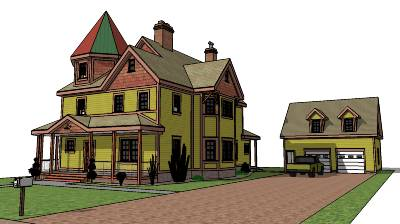
\includegraphics[width=8cm]{warehouse.jpg}
  \caption[A model from a library]{A single model by \emph{Bob1938} from the Timble 3D Warehouse\cite{GoogleWarehouse}, that was found using the search term ``Victorian house''. The time to find and download the model was 30 seconds, a significant improvement on many of the PGM systems presented in this chapter. \copyright Bob1938.}
  \label{fig:warehouse}
\end{figure}

Given such a variety of geometry, some search tools are required to allow users to locate the geometry they require. Most of the commercial websites such as \emph{Trimble Warehouse}\cite{GoogleWarehouse} or Turbosquid use text based search, an example result is show in Fig.~\ref{fig:warehouse}. However searching large collections of 3D meshes remains a active research area. The seminal work in this area by Funkhouser et al.\cite{Funkhouser03} indexes and retrieve meshes by sketches or example models. The rotation invariant properties of \emph{spherical harmonics} are used to construct easily indexed feature vectors. An alternative feature descriptor is given by \cite{Ohbuchi03b}, which uses the low frequencies of the depth map of the rendered object. The rendering stage ensures the system is robust to irregular meshes, such as those which contain holes. 
A different approach is to exploit the continuous variability in a set of models to allow users to explore the set of models interactively, as in \cite{Ovsjanikov11}. For example, users navigate from one airplane mesh to another by indicating that they wish the wings to be further forwards on the fuselage. Recently \emph{fuzzy correspondences} have been introduced as a technique for exploring a library of meshes uses regions of interest that the user specifies on an example model.

Because each model in the library has been manually created, they are free from many of the artifacts that recovered geometry may contain. Furthermore they are free from many technical concerns that come with many of the more general procedural systems, such as termination criteria in the case of shape grammars. However, the user faces several other issues in using this content --- for example, given an existing lot in a city finding a house of the correct style to fit, depends on the contents of the library. Generating a large cityscape may require repeating objects from the library, or mixing meshes of different styles and level of detail. 

%A search engine for 3D models : funkhouser (lots of cites)

%Exploration of continuous variability in collections of 3D shapes\cite{Ovsjanikov11} (-> deformation, more sub-refrefences in related works) Automatic learning of constraints from a set of unlabelled models. User can suggest movement of elements to explore the corpus of existing models. Find curves through deformation space.

%Exploring Collections of 3D Models using Fuzzy Correspondences\cite{Kim12}

%\section{Misc/Applications}
%need to credit:
%Modeling the appearance and behaviour of urban spaces\cite{Vanegas10:MAB}
%There are not a lot documents about the aplpication of procedural modelign?
%Real-time procedural generation of `pseudo infinite' cities\cite{Greuter03}
%EG/carlos overview has references for acceleration of views
%Virtual cities?

\begin{comment} % another time, another place
\section{Evaluation of Procedural Techniques} 

Visual dataflow languages: Criteria for evaluation of visual programming languages. Kipper\cite{Kiper97} (via advances in dataflow programming languages, who says ``criteria included scalability, ease of comprehension, gauging the degree of visual notation of the language, functionally8ity and it's support of the paradigm). Nothing similar for procedural in general?

``When Visual Programs are Harder to Read than Textual Programs'' green, Petre

see google doc ``procedural evaluation'' for ideas, no refs so far.
%http://dx.doi.org/10.1007/978-3-642-16873-4_11
%http://twak.blogspot.co.uk/2009/03/compare.html

A pattern language and architectural theory books for evaluation rather than constructin?\cite{APL}

Pascals papers - several examples, nothing objective.
Grammar papers - proof of expressivness of various classes of grammars.
L-system subject example of whatever they're modeling phylotaxis plant etc... 
Expressivness vs. encoding description?

\cite{Lee08}: evaluation was on three undergrads modeling photos, then two other novice users modeling fixed scenes. not procedural!

Combinatory modeling

Evaluation of expressivness\cite{Chau04}\cite{Gips99}
Harley davidson - do the models conform to brand.
Complexity analysis of evaluating the grammar.
Expressability - 

\cite{Efros99} texture synthesis: several pages of example textures and their results. Similar for all texture synth papers

\cite{Haeberli88}: ``the tradeoff between an expressive system and a ready-made system will always benefit sometusers and leave other unsatisfied''. provides no proof.

\cite{Johnston04} evaluation of visual dataflow langues on page 22 - green and petre. Baroth and Hatysough time improvement in the factor 4.
%The following diagram attempts to place the procedural systems examed in thesis on an axis of automation~\ref{fig:procedural_spectrum}.

\cite{Merrell11} Only an ``informal study'' was performed. Then asked if they prefer assisted version or not.

\cite{Yu11}. example of doign it well - validated study against human designed scenes with the same input.

\cite{Vouga12}. theoretical paper with no attempt to build examples to see if they can stand up or not.

%\section{Commercial Procedural Tools}

%While there is an ivory tower of research into procedural modeling in academia, the greatest evidence for systems' applicability to real world problems . Often advancements are made in industry before

%For example the complexity of each frame has risen from the tens of polygons in the 1980's to the tens of millions today\cite{DevelopInsider}
%~\ref{cityengine}
%Bently genComp ~\ref{bentley}
%revit\cite{Revit}
%Rhino\cite{Rhino} and grasshopper

\end{comment}

\section{Summary}
\label{s:readingsSummary}

% we've concentrated on architectural techniques - whre teh work is being done, and relevant to the thesis.


In general there are many axes on which we can classify the work on procedural modeling, such as quantity of human interaction, or applicability to real-time situations. 
%An alternative grouping that may be more insightful is the range of results possible before any human interaction, and the range of results possible after any human interaction. For example both shape grammars and general 3D tools can produce arbitrary geoemtry before the user interacts with them, but once the user's task is finished, the shape finished grammar may still produce a range of designs, while the 3d tools would only create one object. Meanwhile a city simulation system may only be capable of generating a range of cities before the user interacts, but will produce a model of a city given a particular time after user interaction. 
However in this chapter we have introduced one such axis --- a continuum of procedural specialisation from the general purpose to the specific. 

We have given examples examining the range of geometry that may be generated with each system. From general purpose programming languages, that only happen to be used for geometry creation, through complex grammar and inverse procedural techniques, to simply finding the closest possible item of geometry in a library. Unfortunately it is hard to make a quantitive argument about the trade off between power and ease of use over this spectrum. This is due to the difficulty in capturing ease of use information given the wide range of users' abilities (both programming and artistic), and in quantifying the range of results that a system can create. We may imagine some future work in which users create a model with each system in the spectrum, and we then evaluate the time it took the user, the fidelity, and the range of geometry the created model creates.

Complicating matters we have observed an increasing number of cross over systems in recent years --- combining separate parts of this spectrum to increase the utility of the system. For example, 
\begin{itemize}
\item grammars are used in urban reconstruction via inverse modeling to more tightly fit geometry.  
\item the 3D meshes created by tools can be positioned to form a facade using a shape grammar, that itself is implemented in a general purpose programming language.
\item simulation is used to evaluate the results of L-systems to create models of trees. 
\end{itemize}

Given the broad range of geometry synthesis systems available today, users would be well advised to find the most specific technique that has the required flexibility. For example a video game artist may wish to ``synthesise a large set of alien tower blocks'' with a shape grammar, a town planner may wish to ``visualise this area of a city after a 10\% increase in public transport usage'' using simulation techniques, or residents may only care to ``visualise the new statue outside the town hall'' using mesh construction tools. 



In our introduction we stated that in order to be useful, existing procedural systems required users to write computer programs. With this spectrum of proceduralisation, we can see a strong correlation between general, powerful systems and the requirement to write computer programs. The most general geometry creation techniques, Sec.~\ref{s:gppl} to \ref{s:dataFlowProgramming}, require users to program. The type of programming involved was quite varied; we have encountered systems that use a conventional language, a shape grammar, or a data flow graph to specify an algorithm. Conversely, the the most specific techniques, Sec.~\ref{s:simulation} to ~\ref{s:digitalLibraries} do not require any programming. The user is able to generate a smaller variety of geometry, often confined to a single domain. However they are able to create models using a variety of easier to master techniques such as graphical editing (in the case of shape deformation or geometry construction), discrete selection (in the case of digital libraries or combinatory modeling approaches), or by selecting a number of parameters (in the case of simulation systems).

If we start from the premise that we wish to build a system that is as general as possible without writing a computer program in any form, we find the state-of-the-art in the middle of such a spectrum. 

\section{Approach}
\label{s:approachingTheMiddle}

We wish to possess a system that is as expressive as a split shape grammar, or data flow programming system, but inspired by the types of user interface present in the simulation or inverse procedural modeling approaches. Inspiration for a such a system was forthcoming from Havemann's thesis\cite{Havemann:2005:GMM}. This provides some convincing examples that an offset mechanism driven by the straight skeleton was a powerful accompaniment to a written programming language. After studying a variety of man made objects inside and outside an urban environment, it became clear that some generalised offset mechanism could describe many features of man-made geometry.

The straight skeleton has a simulation-like definition, in which a 2D shape is shrunk until it disappears, leaving behind it a subdivision of the original shape. The output is promising because it was closely correlated to the input, and is quite predictable and easy to understand via a user interface. However the skeleton also had some interesting non-trivial outcomes, such as being able to split concave shapes into two, introducing holes into faces, and leaving behind ``arcs'' which form part of the centrelines of a shape. It is these emergent properties that we found we could exploit to create an expressive range of geometry. 

%comapre the crossover from research section to these two sets of properties of the skeleton?

Chapter 3 introduces our detailed examination of the straight skeleton, the kind of events that we observe as it shrinks, and the kind of degeneracies that occur if we are unlucky. We continue to examine how the straight skeleton can be generalised so that it becomes a more powerful modeling tool in more situations, whilst keeping its desirable properties. 

Given a theoretical understanding of the geometry, we continue to apply the skeleton to the domain of urban procedural modeling. The urban domain has several properties which make it ideal for modeling with skeletons. Given the polygonal output required for many tool-chains used to create 3D environments, the straight edges of many architectural forms was appealing. Cityscapes also offer a more semantically and geometrically demanding domain than, for example flora --- \facades{} have constraints such as only locating doors at street level, and unlike procedurally generated botany, the self-intersection of buildings is undesirable. Finally the urban landscape is well documented, which facilitates easy to obtain reference material and comparisons.

Our first application of the straight skeleton to an urban domain was in identifying the centerline of city blocks so that they could be split into lots. Existing systems  assumed a simpler model, in which the block was repeatedly split into two pieces, however such a system was unable to represent the characteristic centrelines. In Chapter 4 we examine a novel technique for the subdivision of city blocks using the straight skeleton. The straight skeleton is combined with geometric construction techniques to give a parameterised algorithm for city lot formation.

We continue into Chapter 5 to apply a generalisation of the straight skeleton to the construction of solid buildings that may be located within such lots. The similarity of the of the straight skeleton to a building's roof is exploited and extended to generate a wide variety of interesting architectural forms. Repeated applications of the skeleton are guided by user defined plans and profiles to generate buildings. The generalisations of the skeletons that we introduce prove to be robust building blocks for a novel yet expressive system.The emergent properties of the skeleton gives very intricate forms simple constructive definitions. These forms prove to be robust enough for large scale cityscape generation, and capable of generating a wide variety of observed urban structures.



%\item{End of chapter 2 ; a comment on the state of the art, what can skeletons do?. What is lacking, why skeletons can make a contribution.}
%\item{Missing an approach section. givecn state of the art from chapter 2, what methods will I use to tackle the problem.}
